\providecommand\forslides{1}

 
%%%%%%%%%%%%%%%%%%%%%%%%%%%%%%%%%%%%%%%%%%%%%%%%%%%%%%%%%%%%%%%%%%%%%%%%%%%%%

\ifnum\forslides=1

  \documentclass{beamer}
  \usepackage{etex}
  \reserveinserts{108}
  \usepackage{animate}
  \renewcommand{\cite}[1]{[Ref in notes]}

\else

  \documentclass[11pt,a4paper,twoside]{report}
  %%%%%%%%%%%%%%%%%%%%%%%%%%%%%%%%%%%%%%%%%%%%%%%%%%%%%%%%%%%%%%%%%%%%%%%%%%%%%
  \usepackage{beamerarticle}
  \usepackage{graphicx}
  \setlength{\parindent}{0in}
  %%%%%%%%%%%%%%%%%%%%%%%%%%%%%%%%%%%%%%%%%%%%%%%%%%%%%%%%%%%%%%%%%%%%%%%%%%%%%
  \renewcommand{\lecture}[2]{\chapter{#1}}
  %%%%%%%%%%%%%%%%%%%%%%%%%%%%%%%%%%%%%%%%%%%%%%%%%%%%%%%%%%%%%%%%%%%%%%%%%%%%%
  \newcommand\NormalArticleFrameTitleMode{%
    \renewcommand{\frametitle}[1]{%
      \marginpar{\raggedright ##1 (\insertframenumber)}%
    }%
  }
  \newcommand\ExercisesArticleFrameTitleMode{
    \renewcommand{\frametitle}[1]{%
      ##1%
    }%
  }
  \NormalArticleFrameTitleMode
  %%%%%%%%%%%%%%%%%%%%%%%%%%%%%%%%%%%%%%%%%%%%%%%%%%%%%%%%%%%%%%%%%%%%%%%%%%%%%
  \renewcommand{\familydefault}{\sfdefault}
  
  %%%%%%%%%%%%%%%%%%%%%%%%%%%%%%%%%%%%%%%%%%%%%%%%%%%%%%%%%%%%%%%%%%%%%%%%%%%%%

\fi

\usepackage{subfigure,amsmath}
\usepackage{float}
\usepackage{subfigure}
\usepackage{verbatim}
% %\usepackage[xindy]{glossaries}
% \usepackage{enumitem}
\usepackage{tikz}
\usepackage{verbatim}
\usepackage{xcolor,colortbl}
\usepackage{acronym}
\usepackage{multicol}
\hypersetup{colorlinks=true}

\acrodef{ML}{Machine Learning}
\acrodef{HCI}{Human-Computer Interaction}
\acrodef{GP}{Gaussian Process}
\acrodef{MVG}{Multi-Variate Gaussian}
\acrodef{SLM}{Statistical Language Model}
\acrodef{NCNM}{Null Category Noise Model}
\acrodef{AE}[A\&E]{Accident and Emergency}
\acrodef{CRP}{Chinese Restaurant Process}
\acrodef{LC}{Liquid Chromatography}
\acrodef{MS}{Mass Spectrometry}
\acrodef{RT}{Retention Time}
\acrodef{DP}{Dirichlet Process}
\acrodef{HDP}{Hierarchical Dirichlet Process}
\newcounter{taskcounter}

\definecolor{highlightcol}{rgb}{1,0.184,0.275}
\newcommand{\focus}[1]{{\textcolor{highlightcol}{\bf #1}}}
\newcommand{\up}[1]{{\textcolor{red}{\bf #1}}}
\newcommand{\down}[1]{{\textcolor{OliveGreen}{\bf #1}}}
\definecolor{yellowhighlighter}{rgb}{1,0.984,0.8}
\definecolor{nicered}{rgb}{1,0,0}
\definecolor{niceorange}{rgb}{1,0.6,0}
\newcommand{\highlightred}[1]{{\textcolor{nicered}{\bf #1}}}
\newcommand{\highlightorange}[1]{{\textcolor{niceorange}{\bf #1}}}
\newcommand{\todo}[1]{{\textcolor{green}{\bf TODO: #1}}}

\newcommand{\bX}{\mathbf{X}}
\newcommand{\bx}{\mathbf{x}}
\newcommand{\bPars}{\boldsymbol\Theta}
\newcommand{\by}{\mathbf{y}}
\newcommand{\blf}{\mathbf{f}}
\newcommand{\bz}{\mathbf{z}}
\newcommand{\bZ}{\mathbf{Z}}
\newcommand{\bpi}{\boldsymbol\pi}   


\graphicspath{{../Code/GP/}{Figures/}{../Code/DP/}}

\newsavebox{\selvestebox}
\newenvironment{task}
  {\stepcounter{taskcounter}
  \newcommand\colboxcolor{F87A17}%
   \begin{lrbox}{\selvestebox}%
   \begin{minipage}[t]{0.15\textwidth}%\dimexpr\columnwidth-2\fboxsep\relax}
   \textbf{TASK [\arabic{taskcounter}]}%
   \end{minipage}%
   \begin{minipage}[t]{0.8\textwidth}%
   }
%   \begin{minipage}[t]{.45\textwidth}
%  Basic Problems of Single-Photon Polymerization:
%  \begin{itemize}
%  \item layer-by-layer type of manufacturing (limits possible geometries)
%  \item suppression through undesired quenching of radicals
%  \item diffraction limits
%  \end{itemize}
% \end{minipage}
  {\end{minipage}\end{lrbox}%
   \begin{center}
   \fcolorbox[HTML]{\colboxcolor}{FFCC99}{\usebox{\selvestebox}}
   \end{center}}

\newcommand{\LectureTitlePage}{%
    % \setcounter{framenumber}{0}
    \global\def\inserttitle{{Lecture \insertlecturenumber: \insertlecture}}
    \global\def\insertshorttitle{{Lecture \insertlecturenumber: \insertlecture}}
    % \global\def\insertdate{\lecturedate}
    % \global\def\insertshortdate{\lecturedate}
  \titlepage
}

\AtBeginLecture{
    \begin{frame}[plain]
      \LectureTitlePage
    \end{frame}
}
\setbeamertemplate{caption}[numbered]

\title{Non-parametric Bayesian Methods in Machine Learning}
\author{Dr. Simon Rogers\\School of Computing Science\\University of Glasgow\\simon.rogers@glasgow.ac.uk\\@sdrogers}

% \includeonlylecture{Dirichlet}
\includeonlylecture{Metabolomics,hdp}

\begin{document}

\mode<all>

\begin{frame}
	\titlepage
\end{frame}

\mode<all>

%% Outline.tex
\begin{frame}
	\frametitle{Outline}
	\begin{itemize}
		\item {\bf FIX ME AT THE END}
		\item (My) Bayesian philosophy
		\item Gaussian Processes for Regression and Classification
		\begin{itemize}
			\item GP preliminaries
			\item Classification (including semi-supervised)
			\item Regression application 1: clinical (dis)-agreement
			\item Regressopn application 2: typing on touch-screens
		\end{itemize}
		\item Dirichlet Process flavoured Cluster Models
		\begin{itemize}
			\item DP preliminaries
			\item Idenfitying metabolites
			\item (if time) Cluster models for multiple data views
		\end{itemize}
	\end{itemize}
\end{frame}

\begin{frame}
	\frametitle{About me}
	\begin{itemize}
		\item I'm not a statistican by training (don't ask me to prove anything!).
		\item Education:
		\begin{itemize}
			\item Undergraduate Degree: Electrical and Electronic Engineering (Bristol)
			\item PhD: Machine Learning Techniques for Microarray Analysis (Bristol)
		\end{itemize}
		\item Currently:
		\begin{itemize}
			\item Lecturer: Computing Science
			\item Research Interests: Machine Learning and Applied Statistics in Computational Biology and \ac{HCI}
		\end{itemize}
	\end{itemize}
	
\end{frame}

\mode<all>

%% Bayesian intro
\lecture{Bayesian Inference}{bayes}

\begin{frame}
	\frametitle{Bayesian Inference}
	Standard setup:
	\begin{itemize}
		\item We have some data $\bX = \{\bx_1,\ldots,\bx_N\}$
		\item We have a model $p(\bX|\bPars)$
		\item We define a prior $p(\bPars)$
		\visible<2->{
			\item We use Bayes rule (and typically lots of computation) to compute (or estimate) the posterior:
			\[
				p(\bPars|\bX) = \frac{p(\bX|\bPars)p(\bPars)}{p(\bX)}
			\]
		}
	\end{itemize}
\end{frame}

\begin{frame}
	\frametitle{Why Be Bayesian?}
	\begin{itemize}
		\item<2->Ability to incoroporate prior information?
		\item<3->Ability to compute posterior densities (combine prior with likelihood)?
		\item<4->Ability to compare models via marginal likelihood?
		\item<5->For me: the ability to integrate out model parameters completely\ldots
	\end{itemize}
\end{frame}


\begin{frame}
	\frametitle{Why be Bayesian?}
	\begin{itemize}
		\item We're often not interested in parameter values
		\item We're normally interested in something that is a function of the parameter values e.g.:
		\begin{itemize}
			\item Within \ac{ML} we are often interested in making predictions (predicing $y_*$ from $\bx_*$).
			\item This will often require values of some parameters $\bPars$
			\item Being Bayesian allows us to \emph{average} over uncertainity in parameters when making predictions:
			\[
				p(y_*|\bx_*,\bX) = \int p(y_*|\bx_*,\bPars)p(\bPars|\bX)~d\bPars
			\]		
		\end{itemize}
		\item This for me, is the biggest Bayesian selling point!
	\end{itemize}
\end{frame}

\mode<all>

\input{GPIntro}

\mode<all>
% CHI keyboard work

\lecture{Application: Touchscreen typing}{Touchscreen}

\begin{frame}
	\frametitle{Typing on touchscreens}
	\begin{itemize}
		\item Most people have smartphones
		\item Most smartphones have touchscreens
		\item Touchscreens are small
		\item Keyboards on touchscreens are small
		\item Typing on them is hard!
		\begin{itemize}
			\item \ldots but people type on them a lot
		\end{itemize}
	\end{itemize}
\end{frame}

\begin{frame}
	\frametitle{Background 1: Why is it hard?}
	\begin{itemize}
		\item Occlusion of target by finger
		\item `fat finger' problem
		\item Small targets
		\item Demo: \url{http://bit.ly/1nBws97}
		\visible<2->{
			\item Quite a bit of work in this area:
			\begin{itemize}
				\item Holz and Baudisch
				\item Henze (100,000,000 taps)
			\end{itemize}
			\item Collecting data is fairly easy
			}
	\end{itemize}
\end{frame}

\begin{frame}
	\frametitle{Background 2: All users are different}
	\begin{figure}[tbh]
		\centering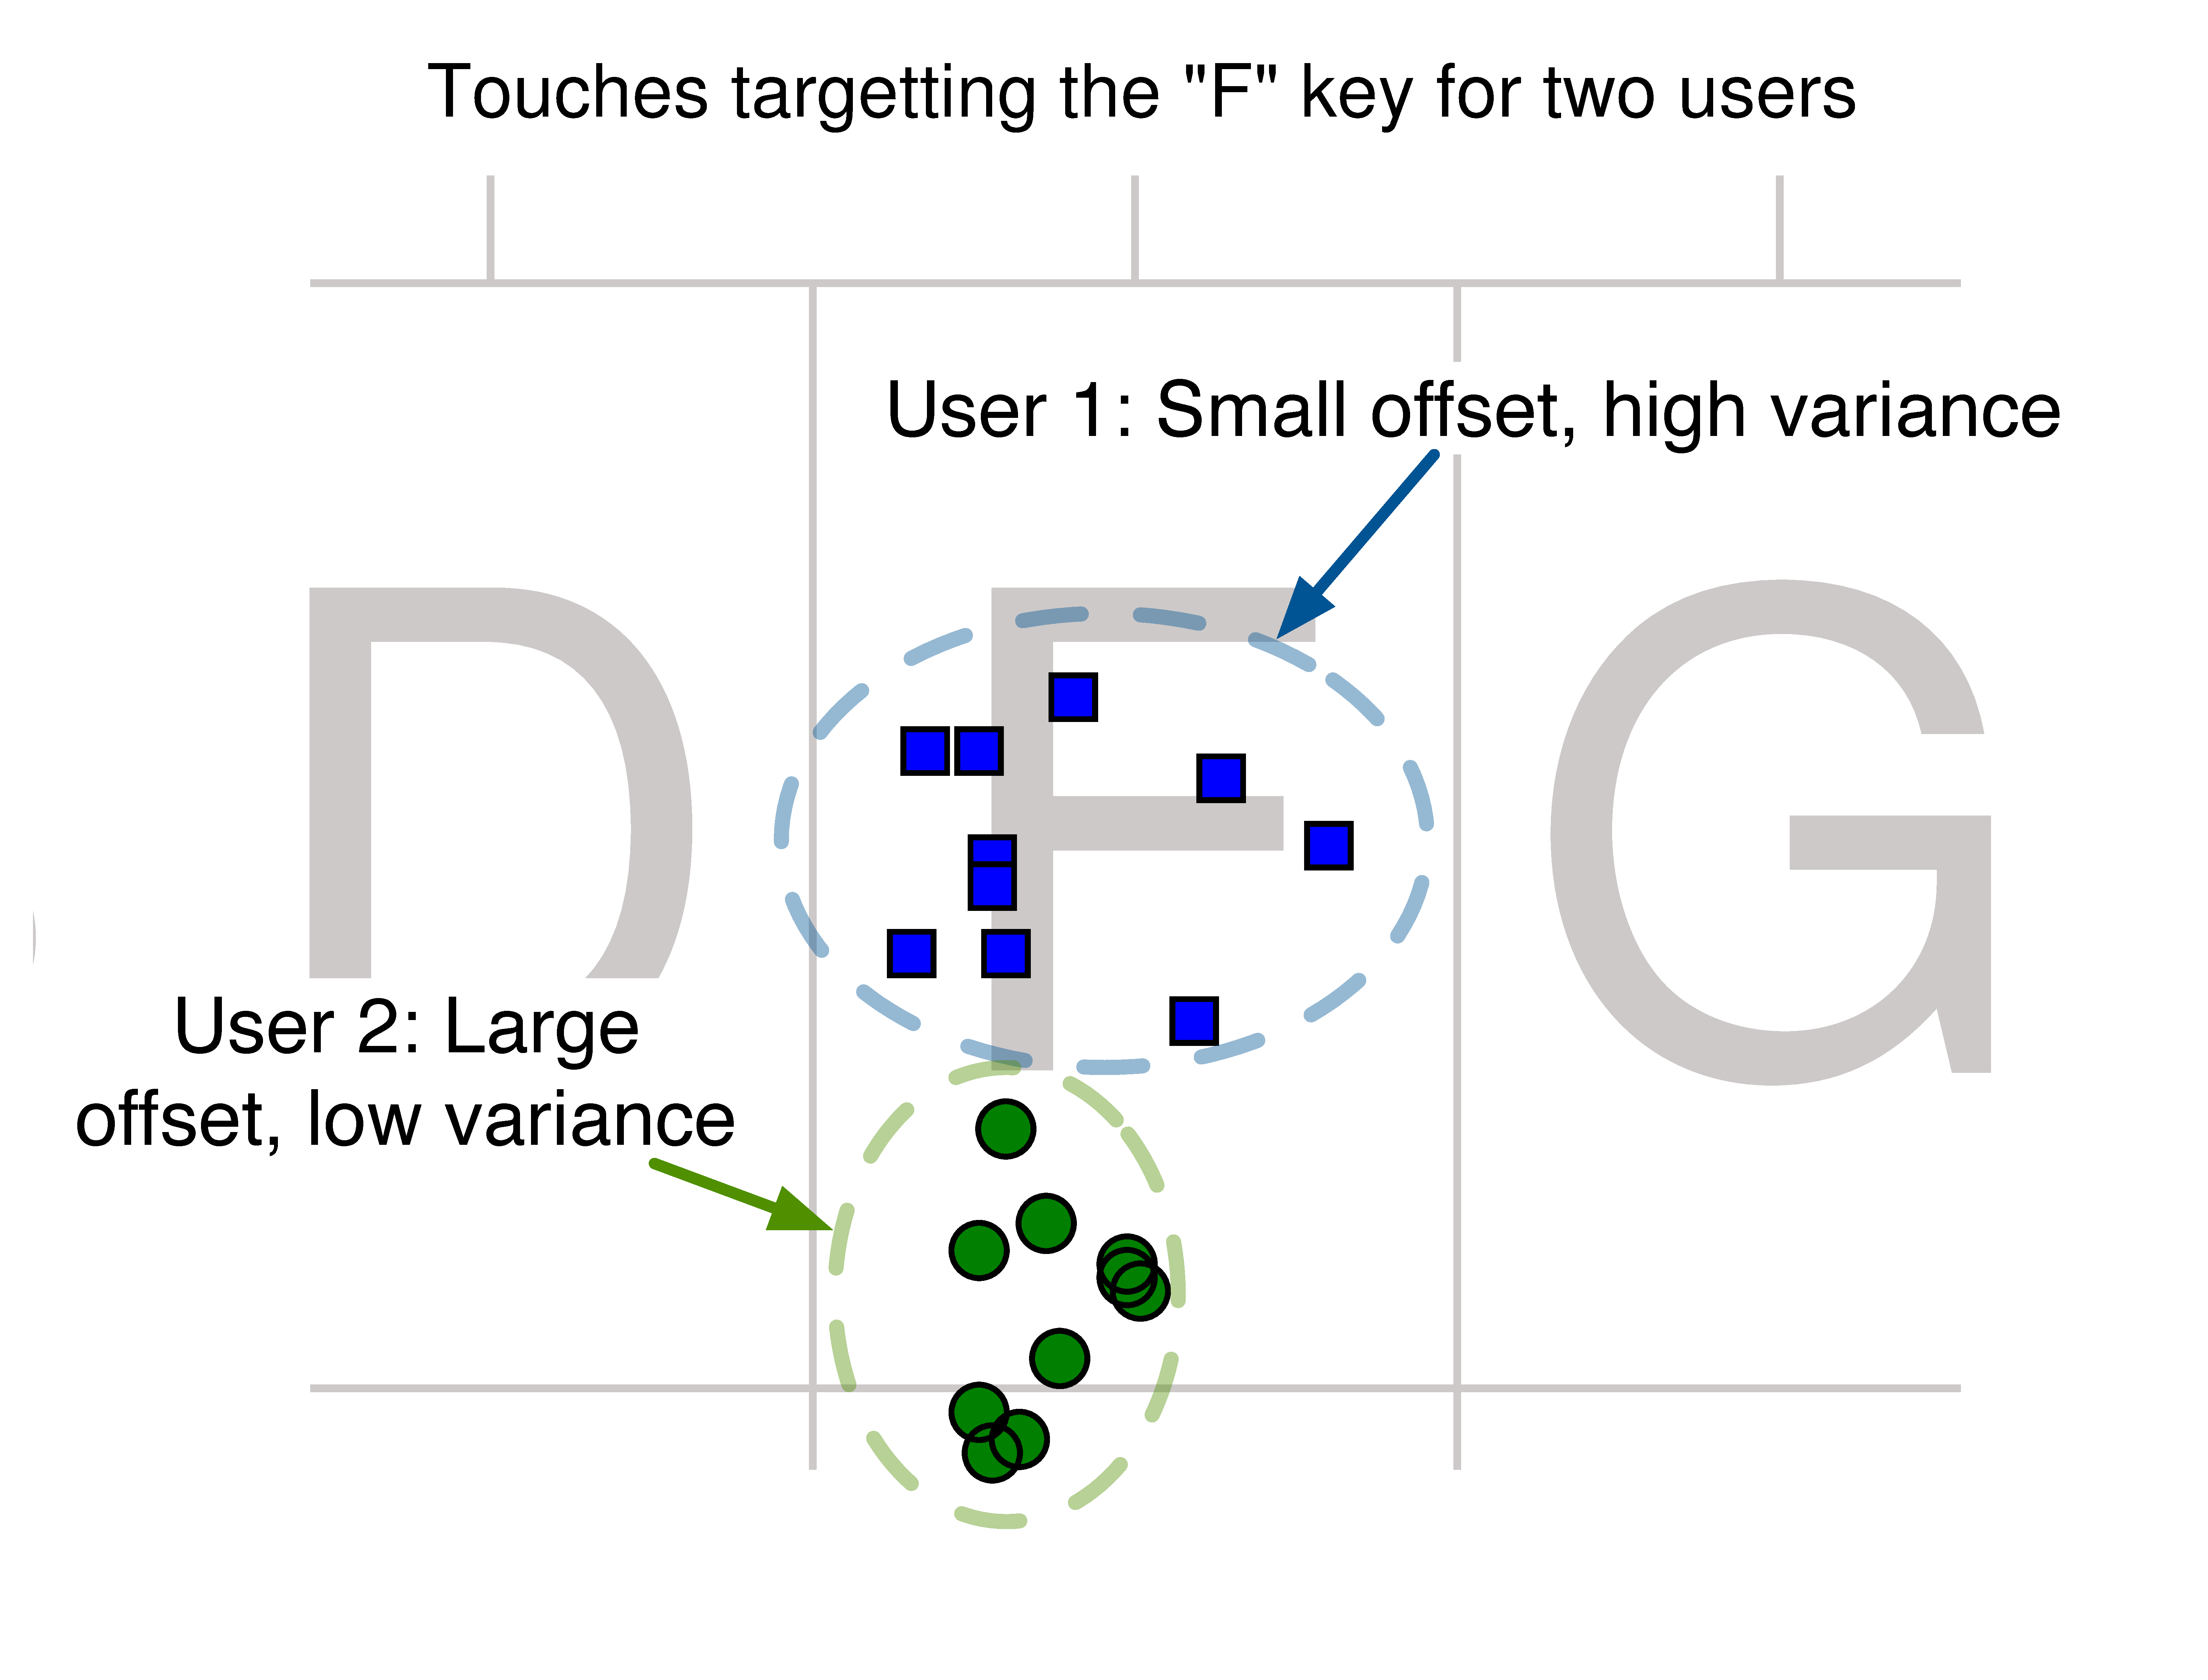
\includegraphics[width=0.8\linewidth]{two_users_annotated.pdf}
		\centering\caption{\label{fig:two_users_annotated}Touches recorded by two users aiming for the `F' key. User 2 has high bias and low variance, user 1 has low bias and high variance.}
	\end{figure}
\end{frame}

\begin{frame}
	\frametitle{Background 3: Current systems (maybe?)}
	\begin{itemize}
		\item Touch is boxed into nearest key.
		\item Key ID is passed to a \ac{SLM}.
		\item \ac{SLM} is made up of probabilities of observing certain character strings (from large text corpora).
		\item \ac{SLM} can swap characters to make the character string more likely.
		\begin{itemize}
			\item e.g. `HELLP $\rightarrow$ HELLO'
		\end{itemize}
	\end{itemize}
\end{frame}


\begin{frame}
	\frametitle{Our idea}
	\begin{itemize}
		\item There is a lot of uncertainty present in touch (bias and variance)
		\item Boxing a touch into a key is probably bad
		\item Why can't we pass a \emph{distribution} to the \ac{SLM}?
		\begin{itemize}
			\item Pass the uncertainty onwards
			\item Being Bayesian!
		\end{itemize}
		\visible<2->{
			\item Can use a user specific GP regression model to predict target from input touch.
		}
	\end{itemize}
\end{frame}

\begin{frame}
	\frametitle{The model}
	\begin{itemize}
		\item We use independent GP regressions for predicting $x$ and $y$ offsets.
		\item Training data:
		\begin{itemize}
			\item Each user typed phrases provided to them.
			\item Data: the $x,y$ location of the recorded touch (i.e. $\bx_n = [x_n,y_n]^T$). Target: the center of the intended key minus the touch (i.e. the offset).
		\end{itemize}
		\item<2-> Used a \ac{GP} with zero mean and a composite covariance:
		\[
			C(\bx_1,\bx_2) = a \bx_1^T\bx_2 + (1-a)\exp \{ -\gamma || \bx_1 - \bx_2 ||^2 \}
		\]
	\end{itemize}
\end{frame}

\begin{frame}
	\frametitle{The model}
	\centering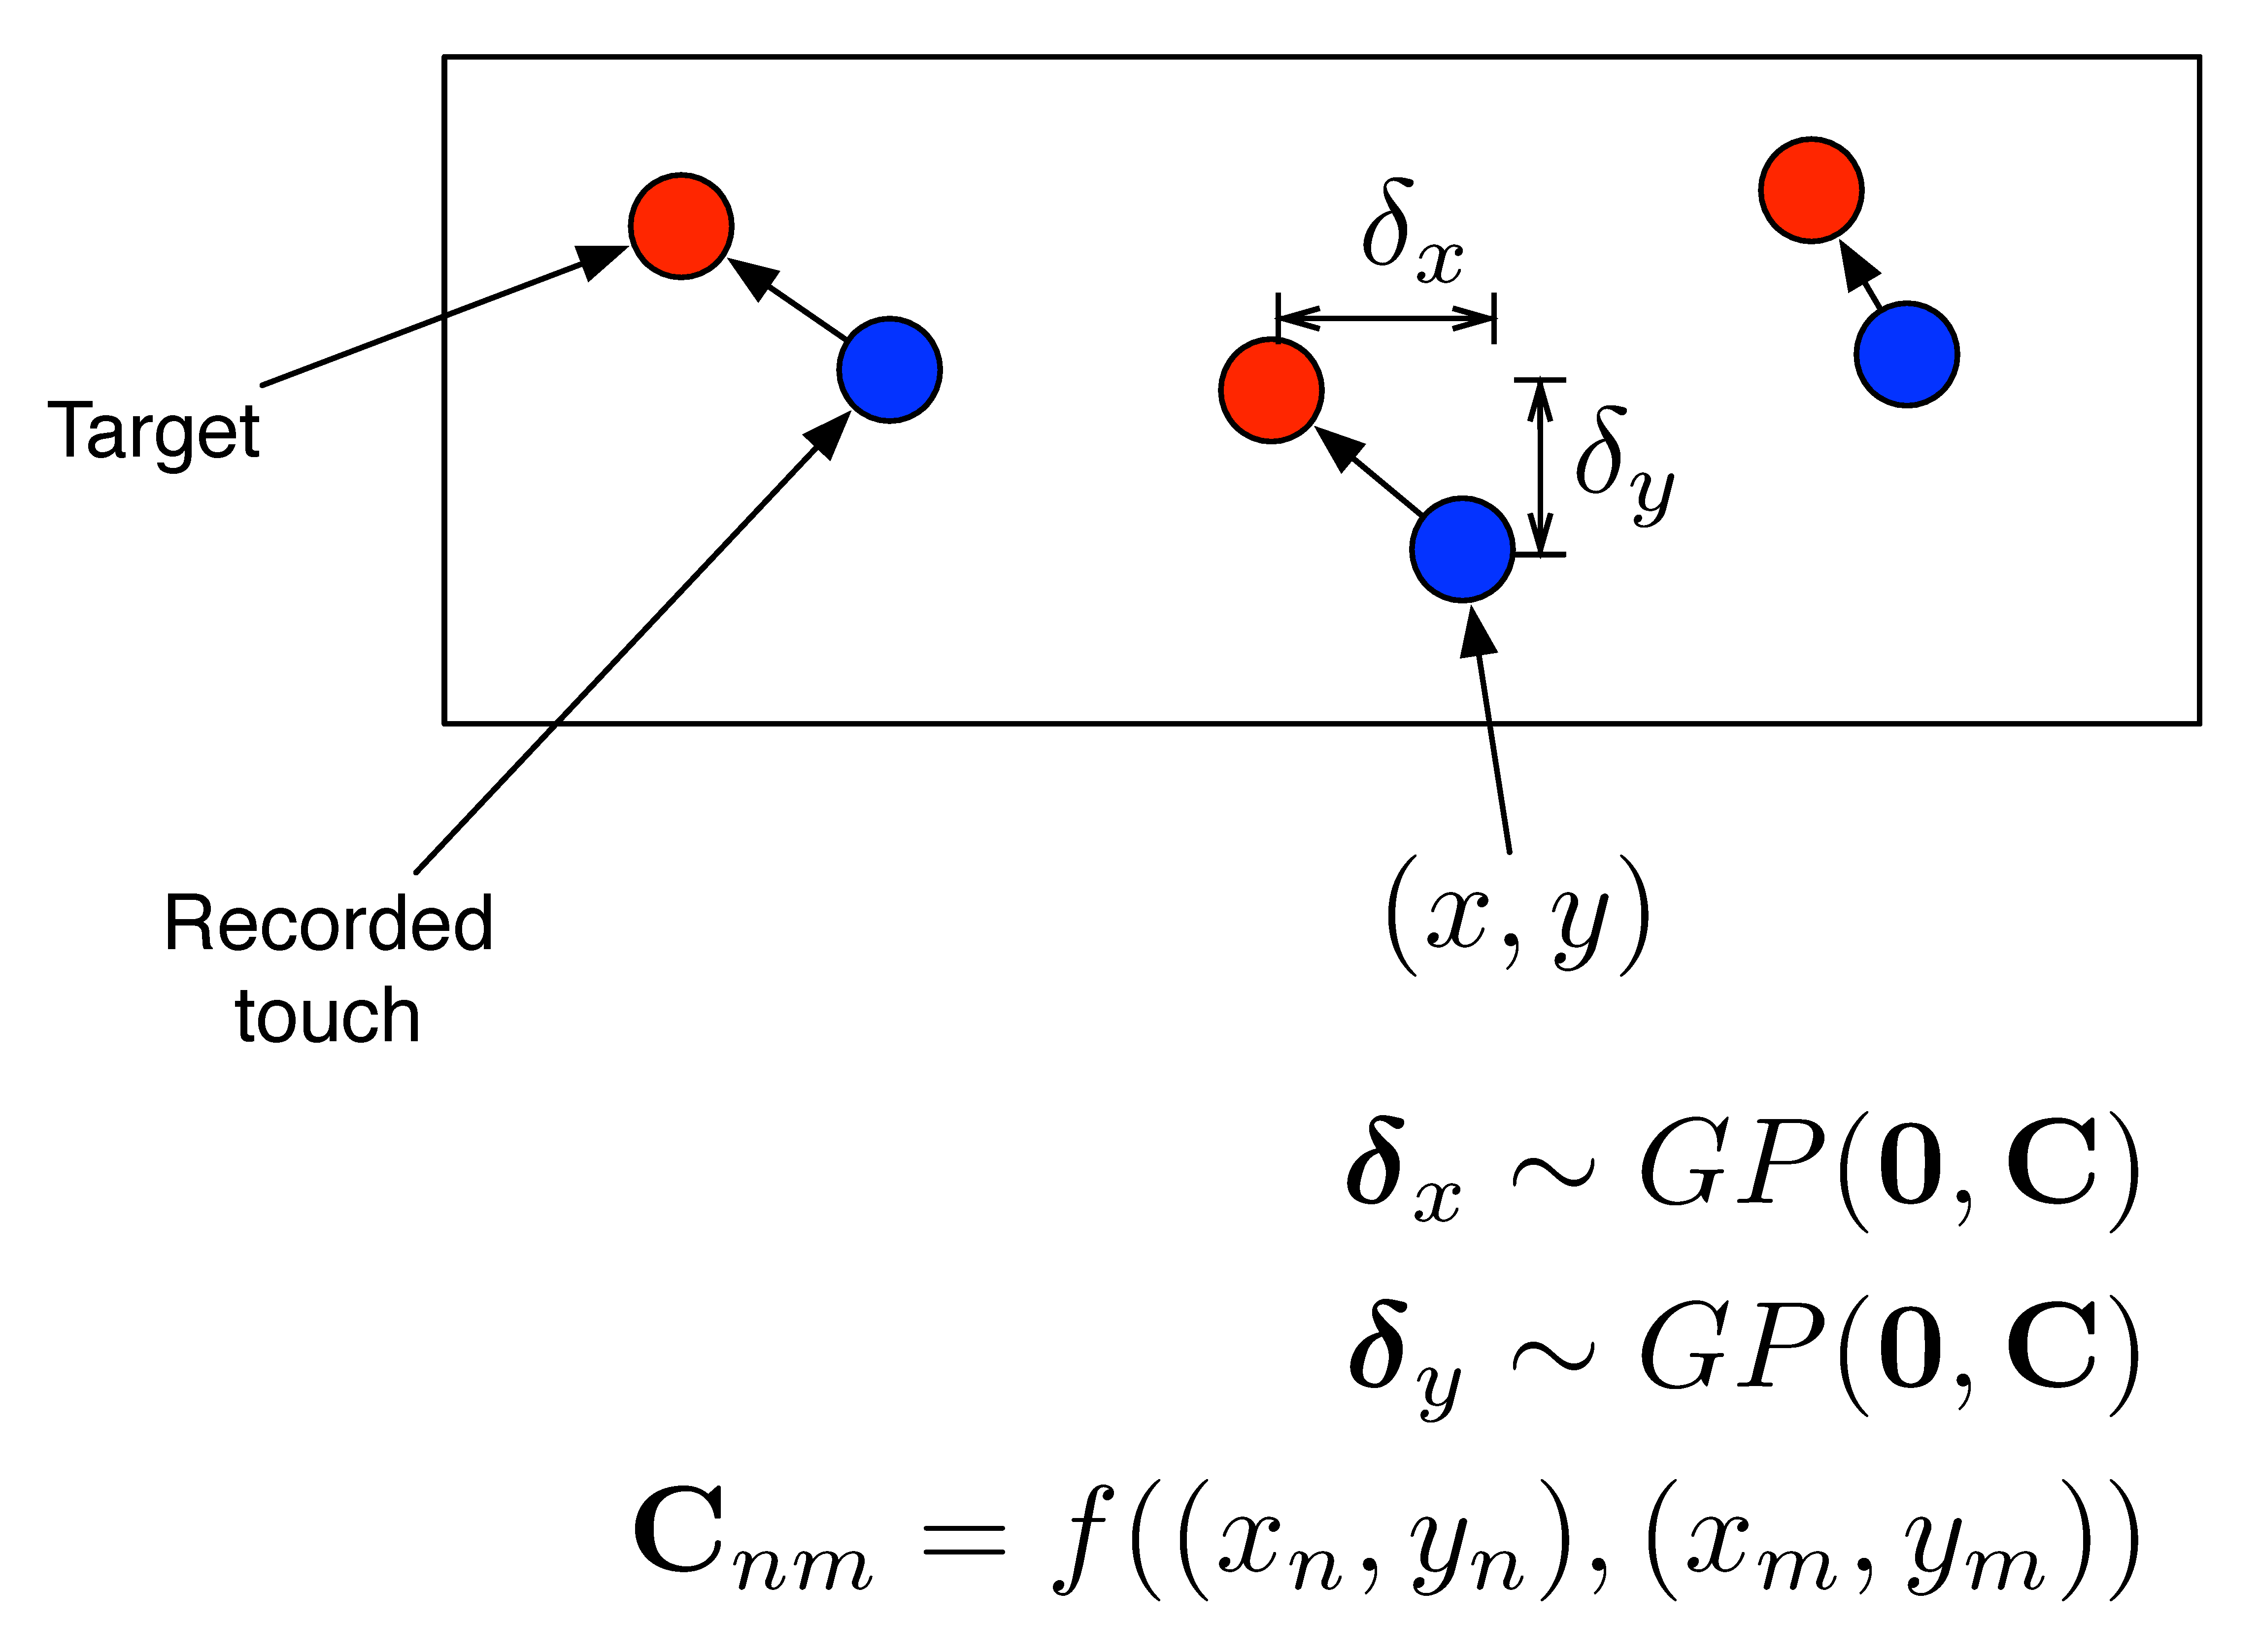
\includegraphics[width=0.7\linewidth]{touchmodel}
	\begin{itemize}
		\item $x$ and $y$ offsets both depend on $x$ and $y$ position of touch
		\item Have also used raw capacitive sensor data as input
		\begin{itemize}
			\item Potentially better (more info) but only accessible on some devices
		\end{itemize}
	\end{itemize}
\end{frame}


\begin{frame}
	\frametitle{System cartoon}
	\begin{figure}
		\centering\includegraphics<1>[width=0.8\linewidth]{cartoon1.pdf}
		\centering\includegraphics<2>[width=0.8\linewidth]{cartoon2.pdf}
		\centering\includegraphics<3>[width=0.8\linewidth]{cartoon3.pdf}
		\centering\includegraphics<4>[width=0.8\linewidth]{cartoon4.pdf}
		\centering\caption{Train GPs to predict the intended touch from an input touch. The flexibility of GPs means that the mean and covariance of the offset can vary across the keyboard.}
	\end{figure}
\end{frame}

\begin{frame}
	\frametitle{System cartoon}
	\begin{figure}[tbh]
		\centering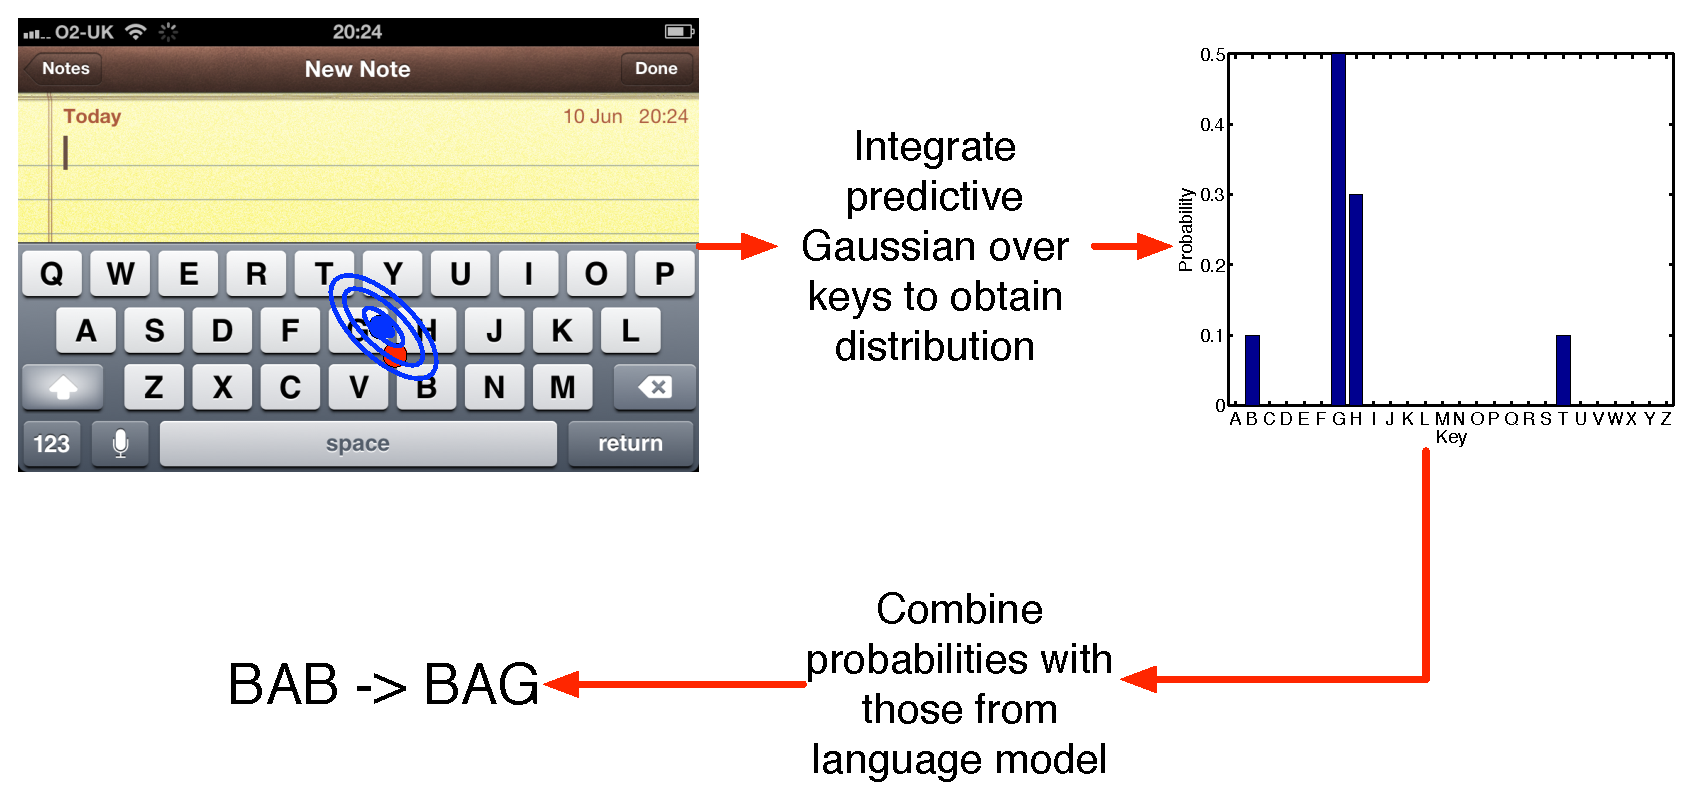
\includegraphics[width=\linewidth]{touchcartoon.pdf}
		\centering\caption{\label{fig:touchcartoon}The complete system}
	\end{figure}
\end{frame}


\begin{frame}
	\frametitle{Video}
	\begin{itemize}
		\item \url{http://www.youtube.com/watch?v=llQI5gV5l74}
	\end{itemize}
\end{frame}

\begin{frame}
	\frametitle{The experiment}
	\begin{itemize}
		\item 10 participants
		\item Calibration data collected for each
		\begin{itemize}
			\item Note: calibration task matters
		\end{itemize}
		\item each did $3\times$ 45 minute sessions, typing whilst sitting, standing and walking. [more details in paper]
		\item Compared:
		\begin{itemize}
			\item GPtype (our system), Swiftkey (commercial Android keyboard), GP only (just offset, no \ac{SLM}), baseline (boxing, no \ac{SLM}).
		\end{itemize}
	\end{itemize}
\end{frame}

\begin{frame}
	\frametitle{Results}
	\begin{figure}[tbh]
		\centering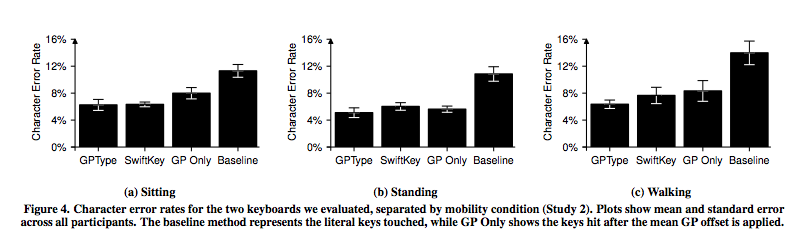
\includegraphics[width=1.0\linewidth]{gptype_results.png}
		\centering\caption{\label{fig:gptype_results}Results of GPType experiment}
	\end{figure}
	\begin{itemize}
		\item GPType marginally (stat sig) better than Swiftkey.
		\begin{itemize}
			\item A {\bf lot} of people work on SwiftKey
		\end{itemize}
		\item Baseline awful!
	\end{itemize}
\end{frame}

\begin{frame}
	\frametitle{Explicit uncertainity control}
	\begin{itemize}
		\item In GPType, uncertainity is handled implicitly
		\item As user typing becomes more uncertain, more power given to language model
		\item Could users \emph{explicitly} control this?
		\begin{itemize}
			\item Certain inputs: no \ac{SLM} control (slang, names, etc)
			\item Uncertain inputs: high \ac{SLM} control
		\end{itemize}
		\item Use pressure to control certainty:
		\begin{itemize}
			\item High pressure: high certainty
			\item Low pressure: low certainty
		\end{itemize}
	\end{itemize}
\end{frame}

\begin{frame}
	\frametitle{Do users know when \ac{SLM} will fail?}
	\centering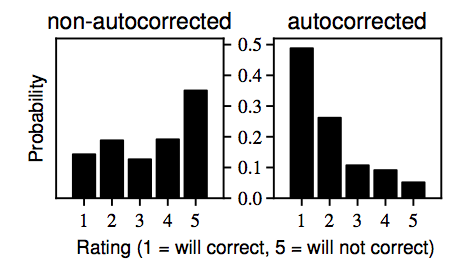
\includegraphics[width=\linewidth]{autocorrect}
	\begin{itemize}
		\item Users given phrases and asked whether they thought autocorrect would change them incorrectly
		\item Users quite good at understanding \ac{SLM} failings
	\end{itemize}
\end{frame}

\begin{frame}
	\frametitle{ForceType}
	\centering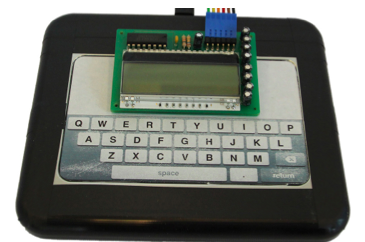
\includegraphics[width=0.6\linewidth]{forcetype}
	\begin{itemize}
		\item Modified Synaptics Forcepad
		\item Pressure mapped to Gaussian variance (no \ac{GP})
		\item System explained to users
		\item Users type phrases with and without forcetype
	\end{itemize}
\end{frame}

\begin{frame}
	\frametitle{ForceType: Results}
	\begin{multicols}{2}
		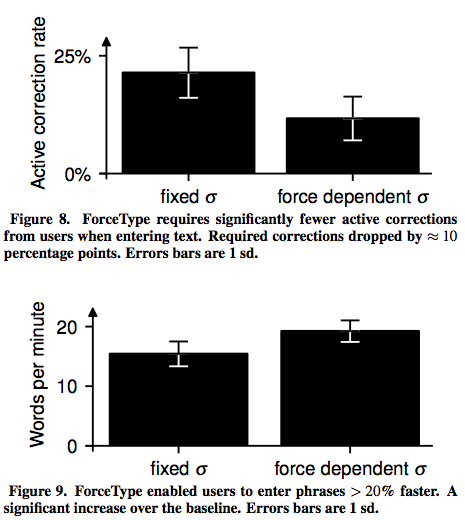
\includegraphics[width=\linewidth]{forcetype_results}
		\newpage
		\vfill
		\begin{itemize}
			\item Forcetype reduced number of corrections performed by users (top)
			\item Forcetype improved overall text entry rate
		\end{itemize}
		\vfill
	\end{multicols}
\end{frame}

\begin{frame}
	\frametitle{Conclusions}
		\begin{itemize}
			\item GP regression is key to the approach: we make no parametric assumptions (what would they be?)
			\item \ldots and get probabilistic predictions
			\item \ldots that can be fed to the \ac{SLM} -- (un)certainity is passed to the \ac{SLM}
			\item Performance is promising
			\item<2->Can also use pressure to provide explicit uncertainty control
			\item<3->More info:
			\begin{itemize}
				\item \url{http://www.youtube.com/watch?v=llQI5gV5l74}
				\item \url{http://pokristensson.com/pubs/WeirEtAlCHI2014.pdf}
				\item Acknowledgements: Daryl Weir, Per Ola Kristensson, Keith Vertanen, Henning Pohl
			\end{itemize}
		\end{itemize}
\end{frame}



\mode<all>
%% GPs for classification and ordinal regression
\lecture{GPs for classification and ordinal regression via the auxiliary variable trick}{Classification}

\begin{frame}
	\frametitle{GPs for Classification and ordinal regression}
	\begin{itemize}
		\item What if our observation model is non-Gaussian?
		\begin{itemize}
			\item Classification:
			\[
				P(y_n=1|f_n) = \int_{-\infty}^{f_n} {\cal N}(z|0,1)~dz = \phi(f_n)
			\]
			\item Logistic Regression:
			\[	
				P(y_n=k|f_n) = \phi(b_{k+1}) - \phi(b_k)
			\]
			\item etc
		\end{itemize}
		\item Analytical inference is no longer possible
		\item I'll cover how to do inference in these models and extensions with the \emph{auxiliary variable trick}
	\end{itemize}
\end{frame}


\begin{frame}
	\frametitle{Binary classification}
	\begin{itemize}
		\item Problem setup: we observe $N$ data / target pairs $(\bx_n,y_n)$ where $y_n\in \{0,1\}$
		\item Place a GP prior on a set of latent variables $f_n$
		\[
			\blf \sim {\cal N}(\mathbf{0},\mathbf{C})
		\]
		\item Use the probit likelihood:
		\[
			P(y_n=1|f_n) = \phi(f_n) = \int_{-\infty}^{f_n} {\cal N}(z|0,1)~dz
		\]
		\item Inference in this form is hard
	\end{itemize}
\end{frame}

\begin{frame}
	\frametitle{Auxiliary Variable Trick}
	\begin{itemize}
		\item Re-write the probit function:
		\begin{eqnarray}
			\nonumber P(y_n=1|f_n) &=& \int_{-\infty}^{f_n} N(z|0,1)~dz\\
			\nonumber & =& \int_{-\infty}^{0} N(z|-f_n,1)~dz\\
			\nonumber &=& \int_{0}^{\infty} N(z|f_n,1)~dz \\
			\nonumber &=& \int_{-\infty}^{\infty} \delta(z>0){\cal N}(z|f_n,1)~dz
		\end{eqnarray}
		where $\delta(expr)$ is 1 if $expr$ is true, and 0 otherwise.
	\end{itemize}
\end{frame}

\begin{frame}
	\frametitle{Auxiliary Variable Trick}
	\begin{itemize}
		\item If we define $P(y_n=1|z_n) = \delta(z_n>0)$ then we have:
		\[	
		P(y_n=1|f_n) = \int_{-\infty}^{\infty} P(y_n=1|z_n)p(z_n|f_n)~dz_n
		\]
		\item and could therefore remove the integral to obtain a model including $z_n$:
		\[
		p(y_n=1,z_n|f_n) = P(y_n=1|z_n)p(z_n|f_n)
		\]
		\item Doing inference in this model (i.e. with additional variables $z_n$) is much easier (but still not analytically tractable)
		\item Note: $P(y_n=0|z_n) = \delta(z_n<0)$
	\end{itemize}
\end{frame}

\begin{frame}
	\frametitle{Example - Gibbs sampling for binary classification}
	\begin{itemize}
		\item An easy way to perform inference in the augmented model is via Gibbs sampling
		\item Sample $z_n | f_n,y_n$:
		\begin{eqnarray}
			\nonumber p(z_n|f_n,y_n=0) &\propto& \delta(z_n<0){\cal N}(z_n|f_n,1)\\
			\nonumber p(z_n|f_n,y_n=1) &\propto& \delta(z_n<1){\cal N}(z_n|f_n,1)
		\end{eqnarray}
		\item<2->Sample $\blf | \bz,\mathbf{C}$
		\[
			 p(\blf|\bz,\mathbf{C}) = {\cal N}(\boldsymbol\mu_f,\boldsymbol\Sigma_f)
		\]
		where
		\[
			\boldsymbol\Sigma_f = \left(\mathbf{I} + \mathbf{C}^{-1}\right)^{-1},~~~ \boldsymbol\mu_f = \boldsymbol\Sigma_f^{-1}\bz
		\]
		\item<2->Repeat ad infinitum
	\end{itemize}
\end{frame}

\begin{frame}
	\frametitle{Example - Gibbs sampling for binary classification}
	\begin{itemize}
		\item To make predictions:
		\begin{itemize}
			\item At each sampling step, do a (noise-free) GP regression using the current sample of $\blf$ to get a density over $f_*$ (Details in a previous slide).
			\item Sample a specific realisation of $f_*$ from this density.
			\item Compute $\phi(f_*)$ (or sample a $z_*$ and then record whether it's $>0$ or not)
			\item Average this value over all Gibbs sampling iterations! 
		\end{itemize}
	\end{itemize}
\end{frame}

\begin{frame}
	\frametitle{Example - binary classification}
	\begin{figure}[tbh]
		\centering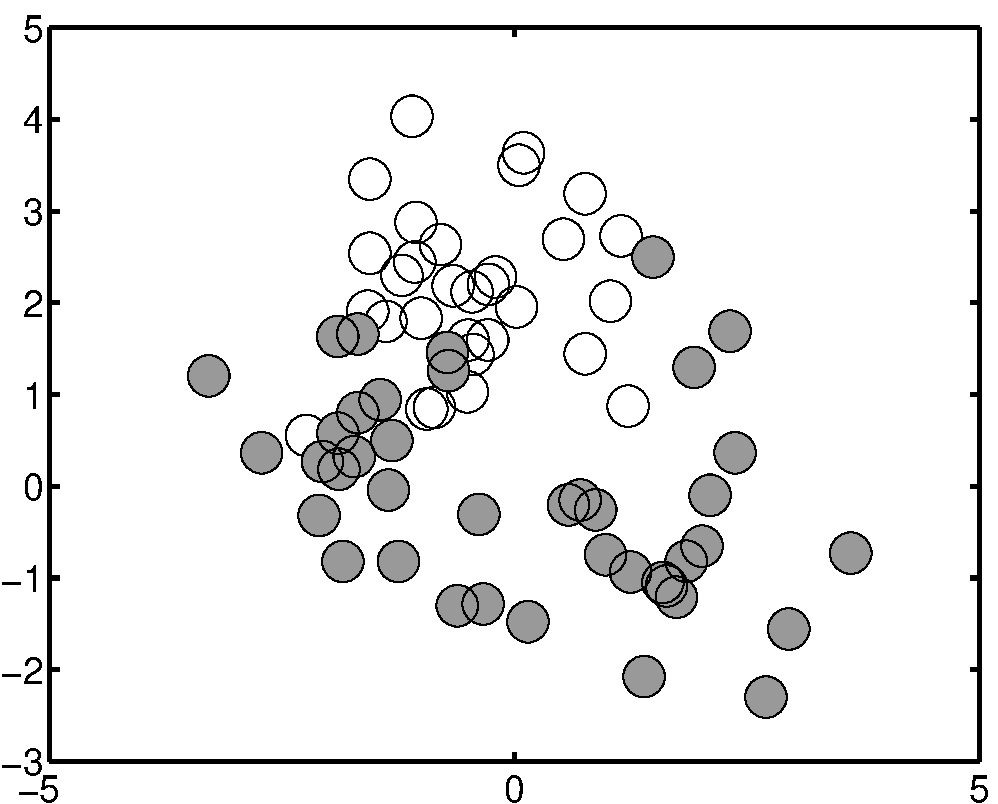
\includegraphics[width=0.7\linewidth]{class_data.pdf}
		\centering\caption{\label{fig:class_data}Some simple classification data}
	\end{figure}
\end{frame}

\begin{frame}
	\frametitle{Example - binary classification}
	\begin{figure}[tbh]
		\centering\includegraphics<1>[width=0.75\linewidth]{gpclass_hyp1_surf.pdf}
		\centering\includegraphics<2>[width=0.75\linewidth]{gpclass_hyp5_surf.pdf}
		\centering\includegraphics<3>[width=0.75\linewidth]{gpclass_hyp10_surf.pdf}
		\centering\caption{\label{fig:binary_results}Predictive probabilities averaged over 1000 Gibbs samples using an RBF covariance. As $\gamma$ is increased, the model overfits.}
	\end{figure}
\end{frame}

\begin{frame}
	\frametitle{Note}
	\begin{itemize}
		\item Inference:
			\begin{itemize}
				\item Gibbs sampling isn't the only option
				\item A popular alternative is Variational Bayes
			\end{itemize}
		\end{itemize}
\end{frame}

\begin{frame}
	\frametitle{Note 2 -- The Generative Process}
	\begin{itemize}
		\item Sometimes it's useful to think of the generative process defined by the model.
		\item In this case, to generate $N$ values of $y_n$ given the associated $x_n$:
		\begin{itemize}
			\item Sample $\blf$ from a \ac{GP} with mean $\mathbf{0}$ and Covariance matrix $\mathbf{C}$.
			\item For each $n=1\ldots N$:
			\begin{itemize}
				\item Sample $z_n\sim {\cal N}(f_n,1)$
				\item If $z_n>0$ set $y_n=1$, otherwise $y_n=0$.
			\end{itemize}
		\end{itemize}
		\item Some examples:
	\end{itemize}
	\begin{center}
		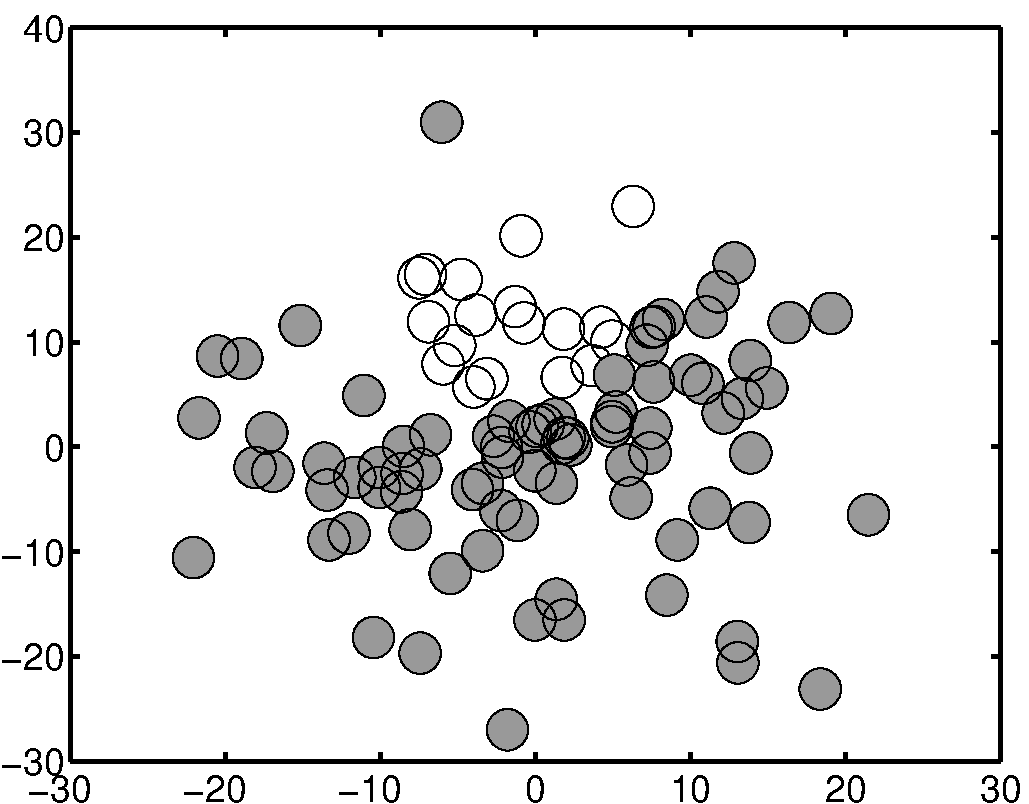
\includegraphics[width=0.3\linewidth]{gendata1.pdf}
		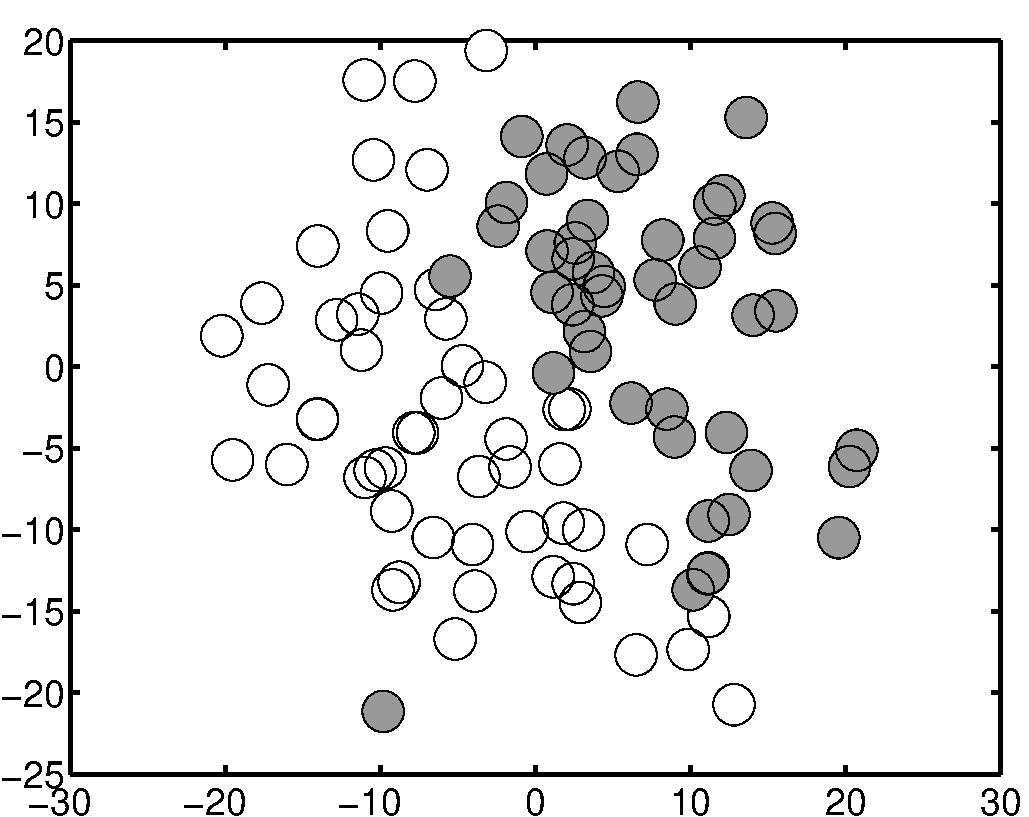
\includegraphics[width=0.3\linewidth]{gendata2.pdf}
		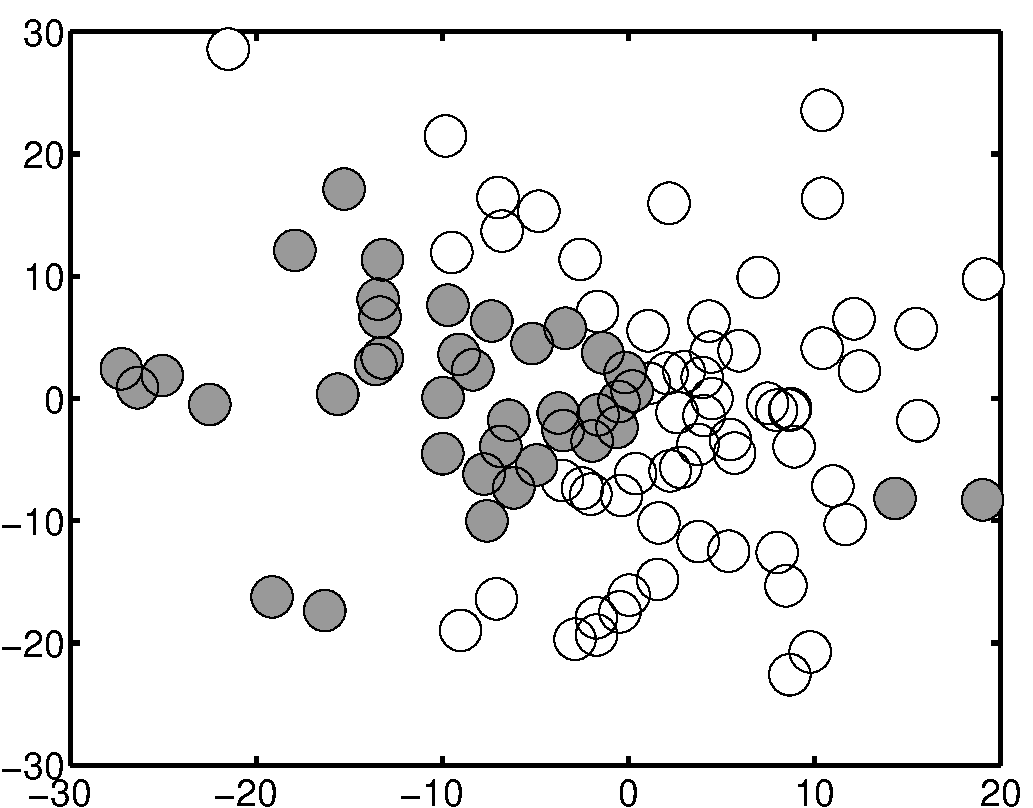
\includegraphics[width=0.3\linewidth]{gendata3.pdf}		
	\end{center}
\end{frame}


\iftasks{
	
	\begin{frame}
		\frametitle{GP classification exercise}
		\begin{task}
			\begin{itemize}
				\item Explore GP binary classification with auxiliary variables using \texttt{gp\_class\_task.m}
				\item Try:
				\begin{itemize}
					\item Generating data from different distributions
					\item Varying covariance function and parameters
					\item Taking more posterior samples
				\end{itemize}
			\item You will also need \texttt{plotClassdata.m} and \texttt{kernel.m}
			\end{itemize}
		\end{task}
		
	\end{frame}

}

\begin{frame}
	\frametitle{A more general idea}
	\begin{itemize}
		\item Models of this form:
		\begin{itemize}
			\item $\blf \sim GP$
			\item $z_n\sim {\cal N}(f_n,1)$
			\item $P(y_n|z_n) = \delta(f(z_n))$
		\end{itemize}
		\item Can be used for more than just binary classification.
		\item<2-> Ordinal Regression:
			\begin{itemize}
				\item $P(y_n=k|z_n)$ is now chopped at both ends:
				\[
					P(y_n=k|z_n) = \delta(b_k<z_n<b_{k+1})
				\]
				\item Gibbs distribution for $z_n$ therefore involves a Gaussian truncated at both ends.
			\end{itemize}
		\item<3->As well as multi-class and semi-supervised classification\ldots
	\end{itemize}
\end{frame}


\begin{frame}
	\frametitle{Multi-class classification}
	\begin{itemize}
		\item The previous treatment can be extended to multiple classes.
		\item For a problem with $K$ classes:
		\begin{itemize}
			\item $K$ GP priors, $K$ $N$-dimensional latent vectors $\blf_k$.
			\item $N\times K$ auxiliary variables $z_{nk} \sim {\cal N}(f_{nk},1)$
			\item And:
			\[
				P(y_n=k|z_{n1},\ldots,z_{nK}) = \delta(z_{nk}>z_{ni} ~~\forall i\neq k)
			\]
		\end{itemize}
		\item<2->Gibbs sampling is similar to the binary case:
			\begin{itemize}
				\item Only tricky bit is efficently sampling from a $K$-dimensionl \ac{MVG} truncated such that the $k$th element is largest.
			\end{itemize}
		\item<3->Details of a Variational Bayes inference scheme in: \href{http://www.mitpressjournals.org/doi/pdf/10.1162/neco.2006.18.8.1790}{Girolami and Rogers 2006}

	\end{itemize}

\end{frame}

\begin{frame}
	\frametitle{Multi-class Example}
	\begin{figure}[tbh]
		\centering\includegraphics<1>[width=0.7\linewidth]{multiclass_data.pdf}
		\centering\includegraphics<2>[width=0.7\linewidth]{multiclass_k1.pdf}
		\centering\includegraphics<3>[width=0.7\linewidth]{multiclass_k2.pdf}
		\centering\includegraphics<4>[width=0.7\linewidth]{multiclass_k3.pdf}
		\centering\caption{\label{fig:multi-class}Multi-class classification example. RBF covariance, $\gamma=1$.}
	\end{figure}
\end{frame}

\begin{frame}
	\frametitle{Semi-supervised Classification}
	\begin{itemize}
		\item In some domains, only a subset of data are labeled [e.g. image classification]
		\begin{figure}[tbh]
			\centering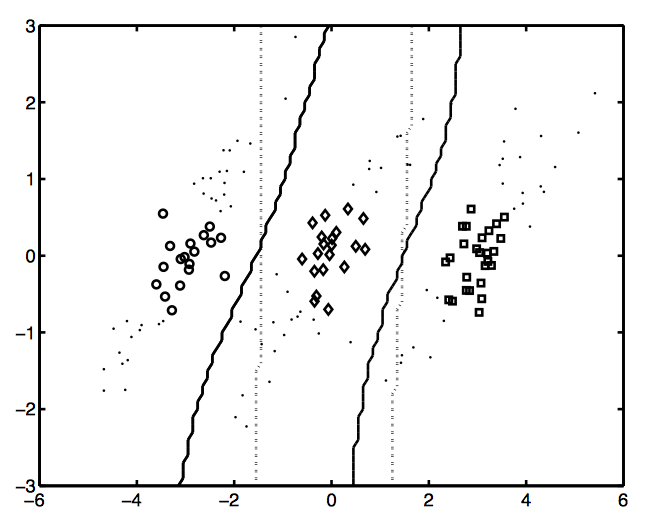
\includegraphics[width=0.5\linewidth]{semisup.png}
			\centering\caption{\label{fig:semisup}A toy semi-supervised classification problem.}
		\end{figure}
		\item Can be overcome using the \ac{NCNM} \href{http://papers.nips.cc/paper/2605-semi-supervised-learning-via-gaussian-processes.pdf}{Lawrence and Jordan 2004}
	\end{itemize}
\end{frame}

\begin{frame}
	\frametitle{The \ac{NCNM}}
	\begin{itemize}
		\item Going back to binary classification, the auxiliary variable trick can be visualised:
		\begin{figure}[tbh]
			\centering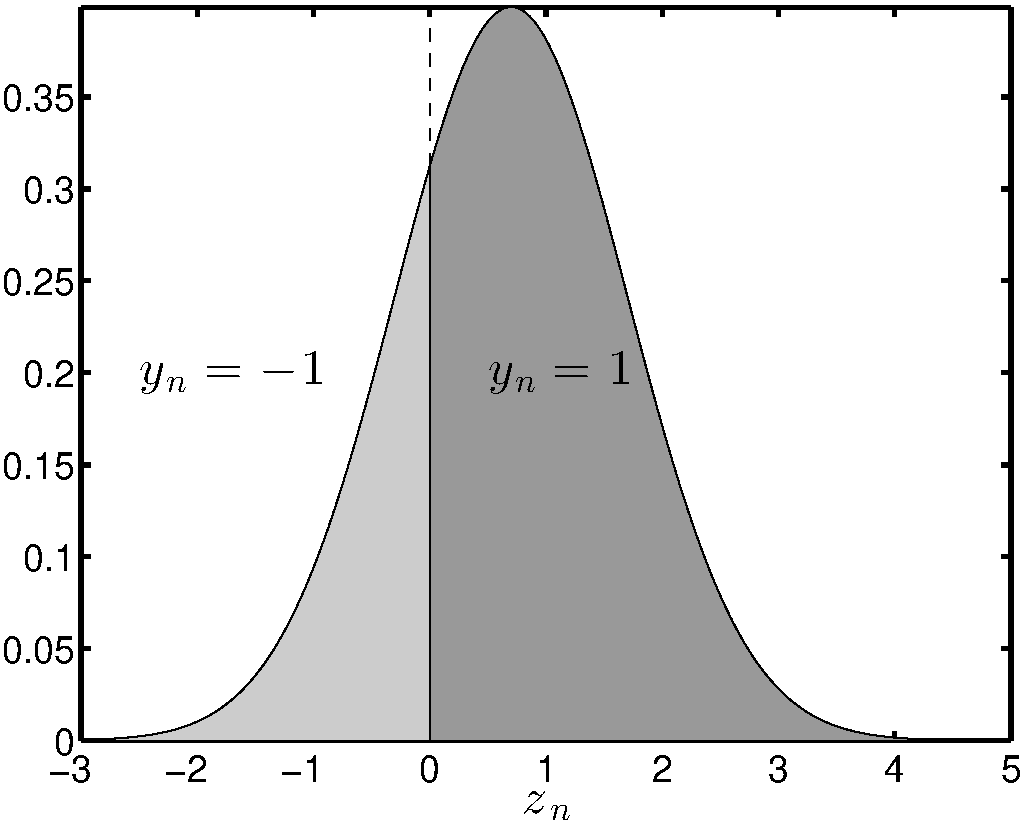
\includegraphics[width=0.7\linewidth]{vis_aux.pdf}
			\centering\caption{\label{fig:vis_aux}Visualisation of the auxiliary variable trick. The Gaussian has mean $f_n$. Note that I'm not calling the classes $\pm 1$.}
		\end{figure}
	\end{itemize}
\end{frame}

\begin{frame}
	\frametitle{The \ac{NCNM}}
	\begin{itemize}
		\item To include unlabeled data, we add a third category, for $y_n=0$:
		\begin{figure}[tbh]
			\centering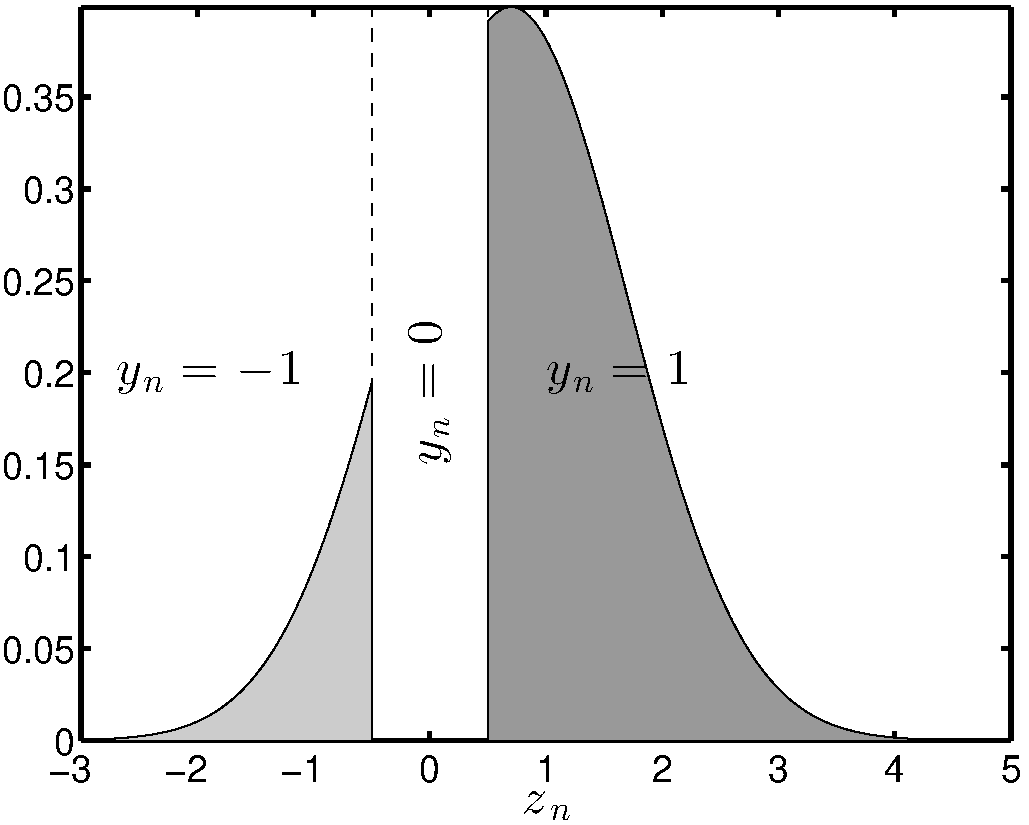
\includegraphics[width=0.5\linewidth]{vis_aux_ncnm.pdf}
			\centering\caption{\label{fig:vis_aux_ncnm}Visualisation of the \ac{NCNM} with a null region of width 1.}
		\end{figure}
		\[
			p(y_n|z_n) = \left\{ 
				\begin{array}{ll}
					\delta(z_n<-a) & y_n = -1\\
					\delta(z_n>a) & y_n = 1\\
					\delta(z_n>-a) - \delta(z_n>a) & y_n=0
				\end{array}
			\right.
		\]
	\end{itemize}
\end{frame}

\begin{frame}
	\frametitle{The \ac{NCNM}}
	\begin{itemize}
		\item The final step is to introduce another set of latent variables.
		\begin{itemize}
			\item $g_n=0$ if $y_n$ is observed (i.e. labeled) and $g_n=1$ otherwise.
		\end{itemize}
		\item And enforce the constraint that no unlabeled points can exist in the null region:
		\[
			P(y_n=0|g_n=1) = 0
		\]
		\item<2->This has the effect of introducing an empty region around the decision boundary
		\begin{itemize}
			\item i.e. pushing the decision boundary into regions of empty space
		\end{itemize}
		\item<3->Inference:
		\begin{itemize}
			\item Gibbs sampling is the same as the binary case except $z_n|f_n,g_n=1$.
			\item This is a mixture of two truncated Gaussians -- sample the component, and then sample $z_n$.
		\end{itemize}
	\end{itemize}
\end{frame}

\begin{frame}
	\frametitle{NCNM Example}
	\begin{figure}[tbh]
		\centering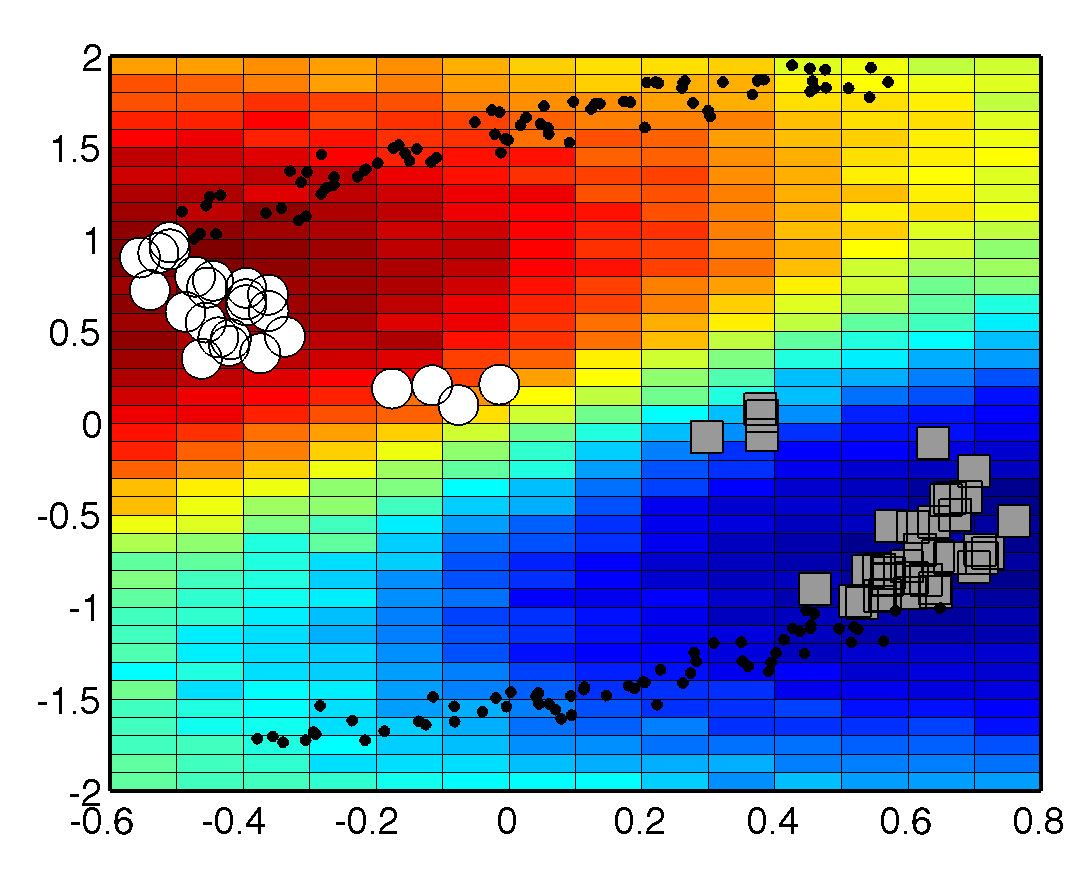
\includegraphics[width=0.8\linewidth]{ncnm_a0.pdf}
		\centering\caption{\label{fig:ncnm_a0}Standard GP classification (unlabeled data ignored)}
	\end{figure}
\end{frame}

\begin{frame}
	\frametitle{NCNM Example}
	\begin{figure}[tbh]
		\centering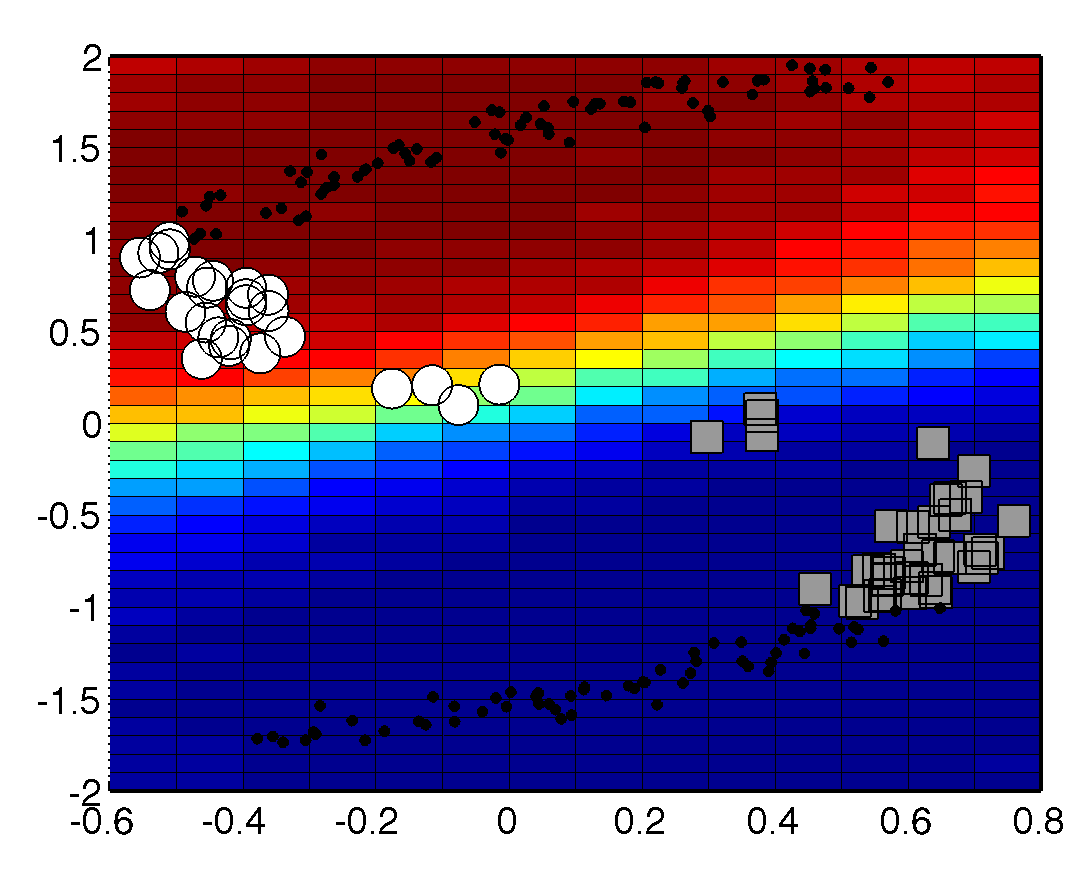
\includegraphics[width=0.8\linewidth]{ncnm_a05.pdf}
		\centering\caption{\label{fig:ncnm_a0.5}NCNM GP classification}
	\end{figure}
\end{frame}

\iftasks{
	\begin{frame}
		\frametitle{NCNM Exercise}
		\begin{task}
			\begin{itemize}
				\item Experiment with the NCNM using \texttt{gp\_ncnm\_task.m}
				\item Setting \texttt{a=0} results in the standard model
				\item Setting \texttt{a>0} uses the NCNM
				\item It's not always easy to get the results you want to see!
			\end{itemize}
		\end{task}
	\end{frame}
}

\begin{frame}
	\frametitle{Multi-class \ac{NCNM}}
	\begin{itemize}
		\item This idea can be extended to the multi-class setting.
		\item See \href{http://jmlr.org/proceedings/papers/v1/rogers07a/rogers07a.pdf}{Rogers and Girolami 2007}
	\end{itemize}
		{\small \[
		P(y_n=k|z_{n1},\ldots,z_{nK}) = \left \{
				\begin{array}{cc}
					\delta(z_{nk} > z_{ni} + a~~\forall i \neq k) & y_n>0\\
					1 - \sum_j \delta(z_{nj} > z_{ni} + a ~~\forall i \neq j) & y_n=0
				\end{array}
			\right.
		\]}
		\begin{figure}[tbh]
			\centering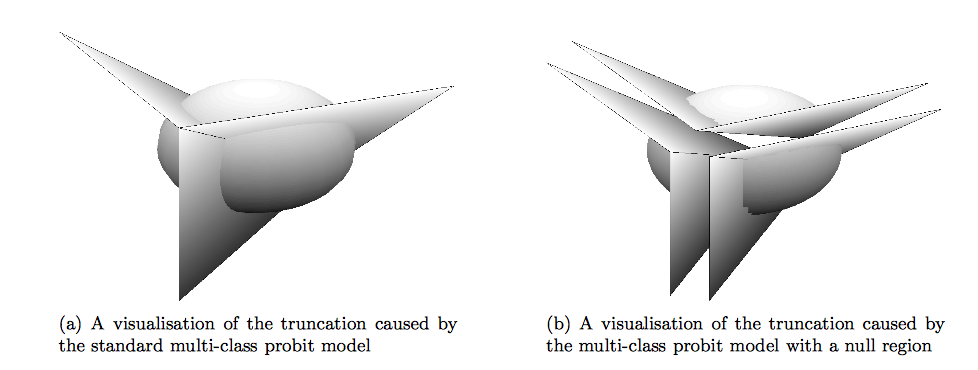
\includegraphics[width=\linewidth]{nullsphere.png}
			\centering\caption{\label{fig:nullsphere}Visualisation of truncation}
		\end{figure}
\end{frame}

\begin{frame}
	\frametitle{Summary}
	\begin{itemize}
		\item \ac{GP} priors aren't restricted to regression.
		\item Analytical solutions aren't possible
		\item Auxiiliary Variable Trick makes inference (via Gibbs sampling or Variational Bayes) straightforward for:
		\begin{itemize}
			\item Binary classification
			\item Ordinal regression
			\item Multi-class classification
			\item Semi-supervised classification (binary and mutli-class)
			\item As well as others (e.g. binary PCA)
		\end{itemize}
	\end{itemize}
\end{frame}


\mode<all>
% Clinical ratings

\lecture{Application: Clinical Ratings}{Clinical}

\begin{frame}
	\frametitle{Clinicians disagree in AandE}
	\begin{itemize}
		\item Patients in \ac{AE} are continually monitored.
		\begin{itemize}
			\item Heart rate
			\item Blood pressure
			\item Temperature
			\item etc
		\end{itemize}
		\item<2-> Based on these hourly observations, clinicians (in a Glasgow hospital) give each patient an ordinal rating
		\begin{itemize}
			\item A (healthy(ish)), B, C, D, E, F (critical)
		\end{itemize}
		\item<3->These ratings are \emph{subjective}
		\begin{itemize}
			\item How do clinicians disagree? (variance? bias?)
		\end{itemize}
		\item<3->More details of this work in \href{http://dx.doi.org/10.1109/JBHI.2013.2252182}{Rogers et al 2013} and \href{http://dx.doi.org/10.1007/s11222-009-9125-z}{Rogers et al 2010}
	\end{itemize}
\end{frame}

\begin{frame}
	\frametitle{Data}
	\begin{itemize}
		\item $c = 1\ldots C$ clinicians.
		\item $p=1\ldots P$ patients.
		\item For patient $p$, we have $T_p$ observations at times $\mathbf{t}_p = [t_{p1},\ldots,t_{pT_p}]^T$.
		\item $y_{\tau c}^p$ is rating at $t_{p\tau}$ ($\{A,B,C,D,E\}$).
		\item The model:
		\begin{itemize}
			\item Patient health is modelled as a GP.
			\item Each clinician has their own offset and precision used to \emph{corrupt} the health function ($q$).
			\item $q$ is binned to produce rating.
		\end{itemize}
	\end{itemize}
\end{frame}

\begin{frame}
	\frametitle{Model}
	\begin{multicols}{2}
		\begin{figure}[tbh]
			\centering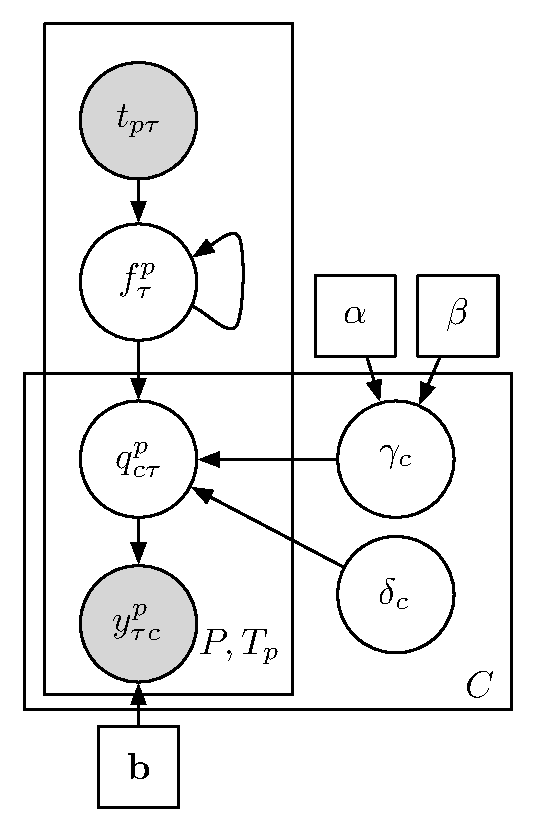
\includegraphics[width=0.9\linewidth]{ClinicalCartoon.pdf}
			\centering\caption{\label{fig:clincartoon}Plates diagram}
		\end{figure}
		\newpage
		\begin{eqnarray}
			\nonumber \blf^p &\sim & {\cal N}(\mathbf{0},\mathbf{C}^p)~~\mbox{[health]}\\
			\nonumber \delta_c &\sim & {\cal N}(0,1)~~\mbox{[offset]}\\
			\nonumber \gamma_c &\sim & {\cal G}(\alpha,\beta)~~\mbox{[precision]}\\
			\nonumber q_{c\tau}^p &\sim & {\cal N}(f_\tau^p + \delta_c,\gamma_c^{-1})\\
			\nonumber P(y_{\tau c}^p=k) &=& \delta(b_k < q_{c\tau}^p < b_{k+1})
		\end{eqnarray}
		Previously auxiliary variables were $z_n\sim {\cal N}(f_n,1)$. This model adds clinician-specific offsets and precisions: $q_{c\tau}^p \sim  {\cal N}(f_\tau^p + \delta_c,\gamma_c^{-1})$.
	\end{multicols}
\end{frame}

\begin{frame}
	\frametitle{Example data generation}
	\begin{figure}[tbh]
		\centering\includegraphics<1>[width=0.8\linewidth]{health.pdf}
		\centering\includegraphics<2>[width=0.8\linewidth]{health_corrupted.pdf}
		\centering\includegraphics<3>[width=0.8\linewidth]{health_corrupted_ratings.pdf}
		\centering\caption{\label{fig:health_example}Example of the generative process described by the model for three clinicans.}
	\end{figure}
\end{frame}

\begin{frame}
	\frametitle{Model inference}
	\begin{itemize}
		\item Gibbs sampling is straightforward
		\item We sample:
		\begin{itemize}
			\item The latent health function for each patient.
			\item The auxiliary variables.
			\item The offset and precision for each clinician.
		\end{itemize}
		\item<2->The offset and precision tell us how the clinicians disagree.
		\item<3->Identifiability: offset for one clinician fixed to 0.
	\end{itemize}
\end{frame}

\begin{frame}
	\frametitle{Results}
	\begin{figure}[tbh]
		\centering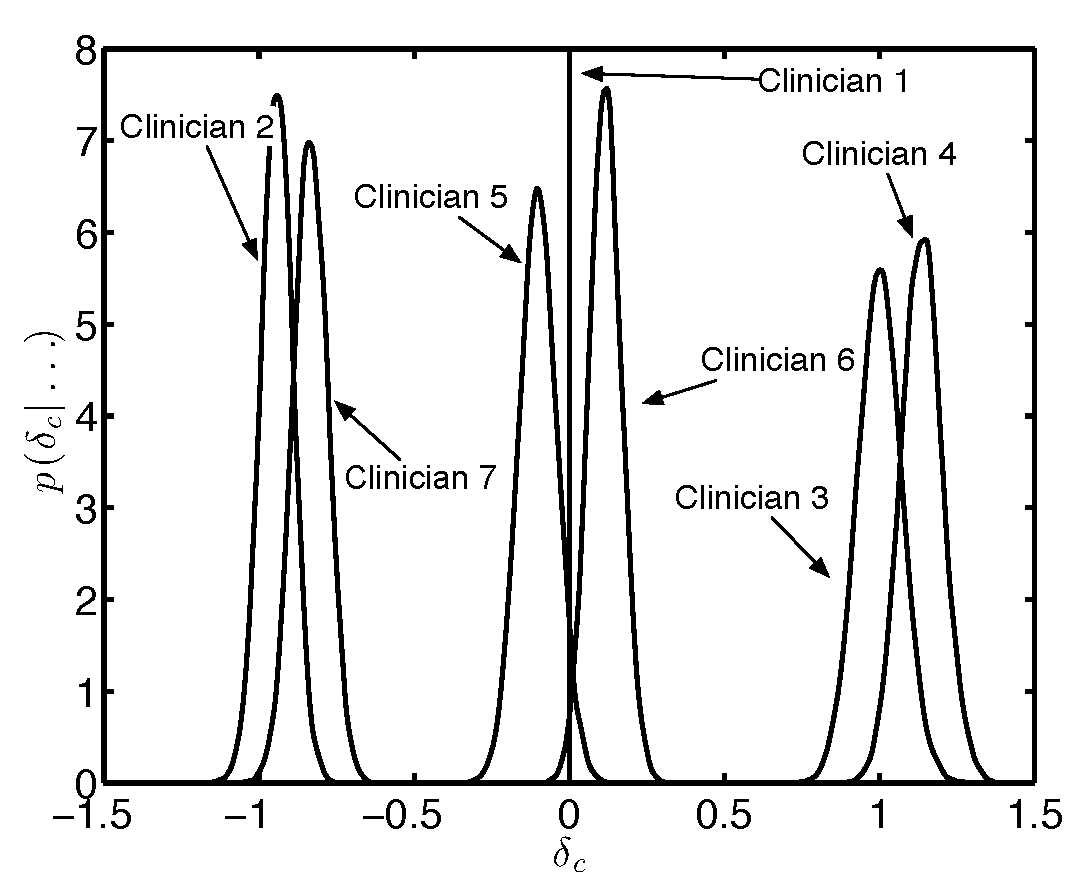
\includegraphics[width=0.8\linewidth]{offset.pdf}
		\centering\caption{\label{fig:offset}Marginal offset posteriors}
	\end{figure}
\end{frame}

\begin{frame}
	\frametitle{Results}
	\begin{figure}[tbh]
		\subfigure[Clinicians 2 and 4]{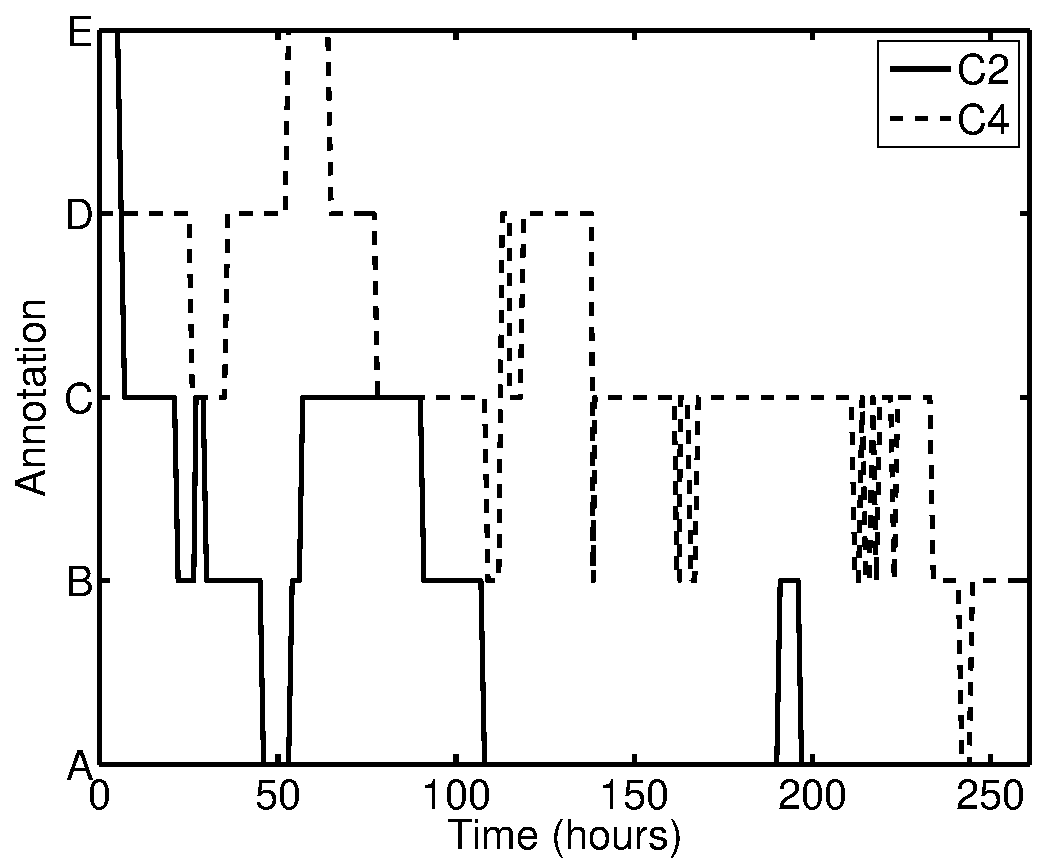
\includegraphics[width=0.45\linewidth]{P2_C24.pdf}}
		\subfigure[Clinicians 3 and 4]{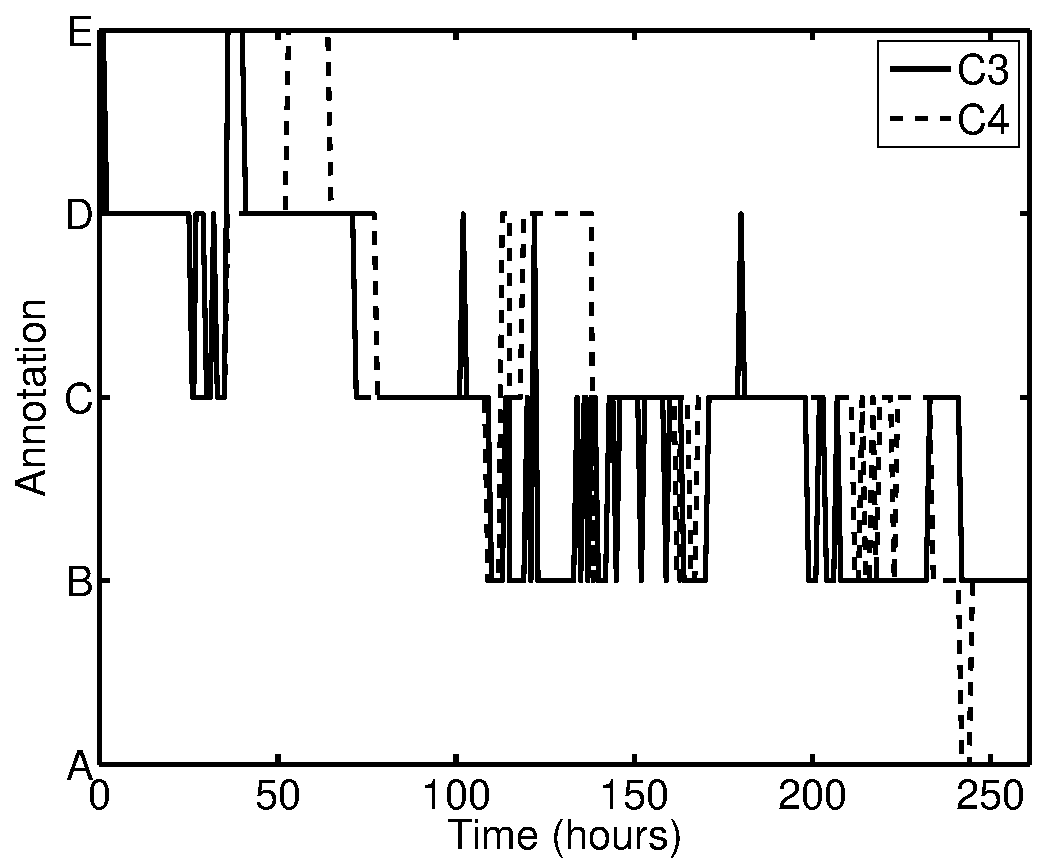
\includegraphics[width=0.45\linewidth]{P2_C34.pdf}}
		\centering\caption{\label{fig:actualratings}Inferred offsets make sense on inspection of the data.}
	\end{figure}
\end{frame}

\begin{frame}
	\frametitle{Results}
	\begin{figure}[tbh]
		\centering\includegraphics[width=0.8\linewidth]{precision_offset_box_17thApril.pdf}
		\centering\caption{\label{fig:clinicalprecision}Marginal precision posteriors. Clinicians 1, 4, and 8 appear to be the least consistent (wrt the majority)}
	\end{figure}
\end{frame}

\begin{frame}
	\frametitle{INSIGHT}
	\begin{itemize}
		\item After the initial annotation, clinicians went through INSIGHT procedure.
		\item The goal was to make ratings more consistent.
		\item If it succeeded, we should see a recuction in offset and increase in precision in the post-INSIGHT data.
	\end{itemize}
\end{frame}

\begin{frame}
	\frametitle{Post-INSIGHT results}
	\begin{figure}[tbh]
		\subfigure[Offsets]{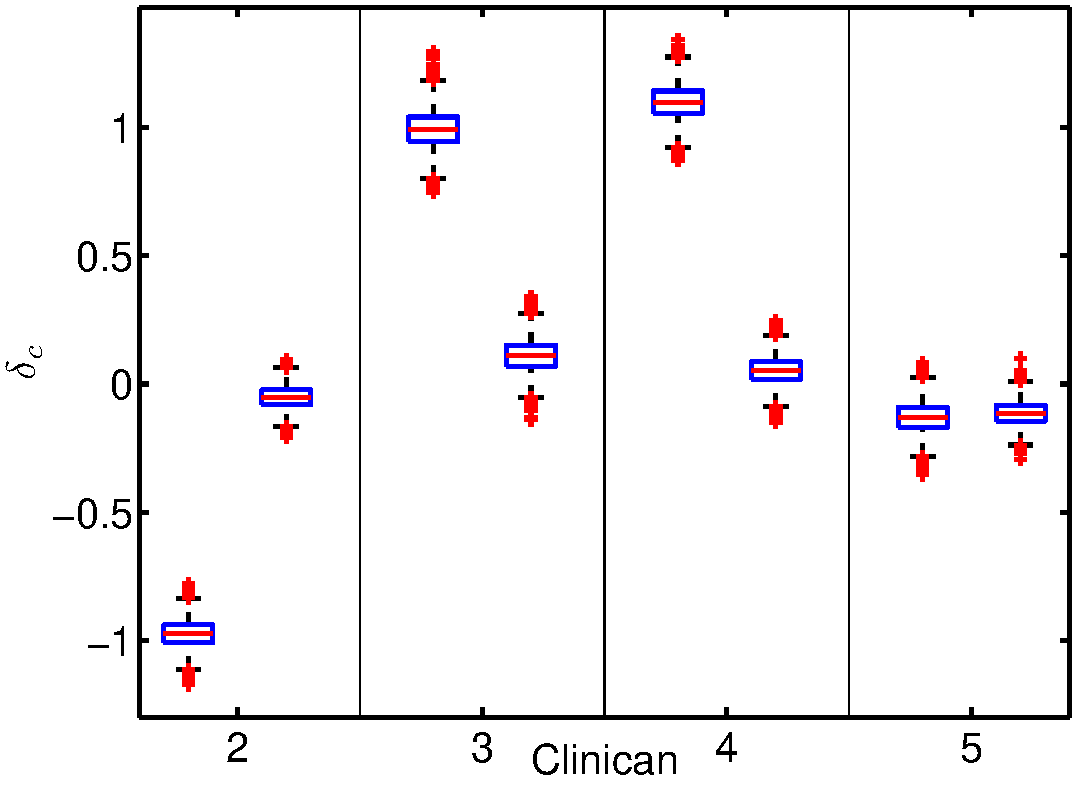
\includegraphics[width=.45\linewidth]{Offset_compare_before_after_17April.pdf}}\hfill
		\subfigure[Precisions]{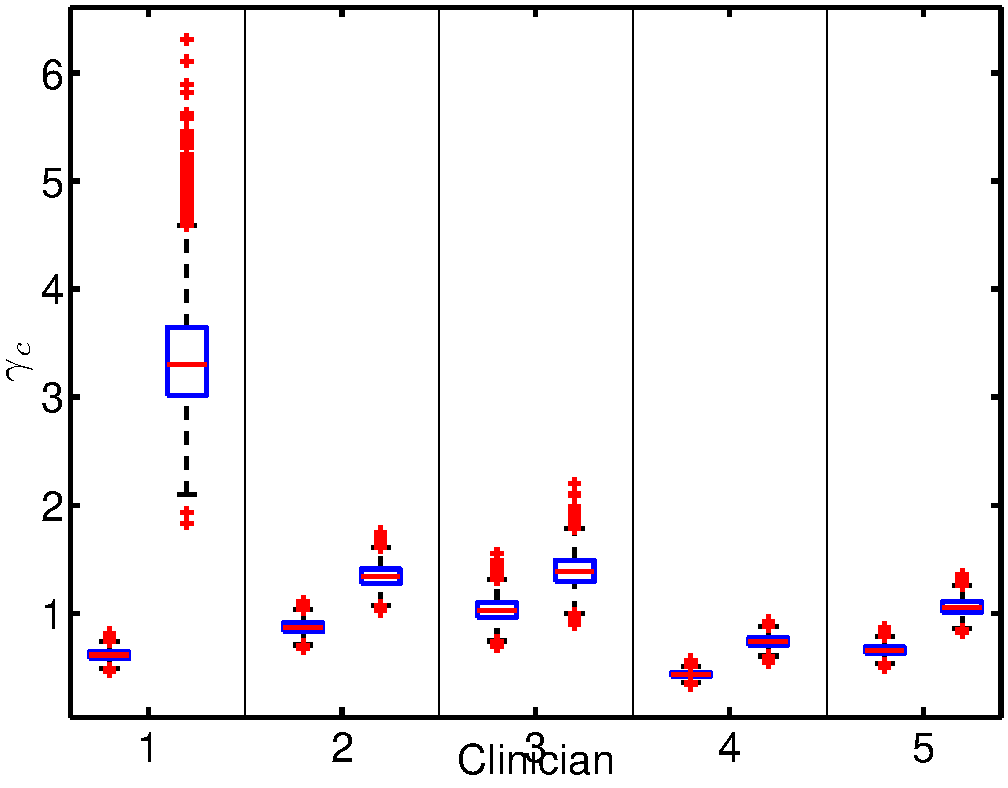
\includegraphics[width=.45\linewidth]{Precision_before_after_April19th.pdf}}
		\centering\caption{\label{fig:clinoffprec}Offsets and precision before and after INSIGHT. Offsets get closer to 0, whilst precision increase suggesting greater agreement amongsth clinicians.}
	\end{figure}
\end{frame}

\begin{frame}
	\frametitle{Inferring category boundaries}
	\begin{itemize}
		\item So far, it has been assumed that all categories are the same size (i.e. the elements of $\mathbf{b}$ are equally spaced).
		\item We can also infer these (with fixed end-points and $\delta_c=0$).
		\item Removes uniform prior assumption over categories.
	\begin{figure}[tbh]
		\subfigure[Before INSIGHT]{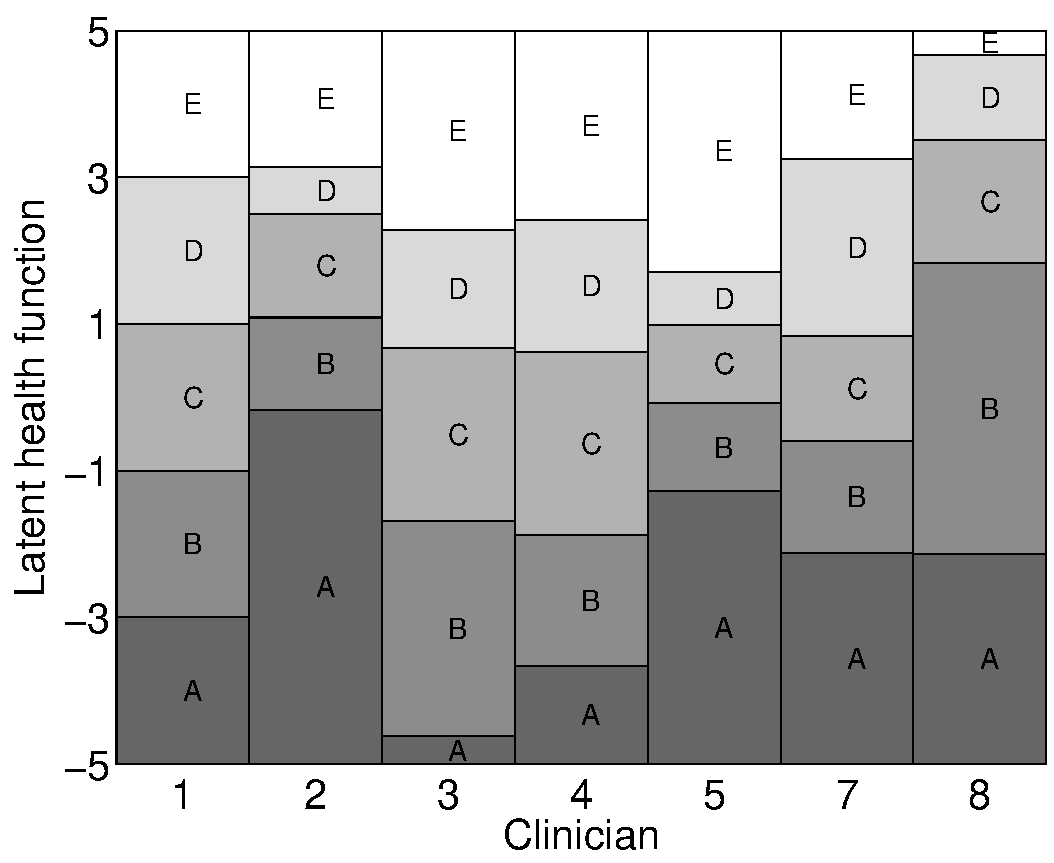
\includegraphics[width=0.45\linewidth]{start_thresh.pdf}}\hfill
		\subfigure[After INSIGHT]{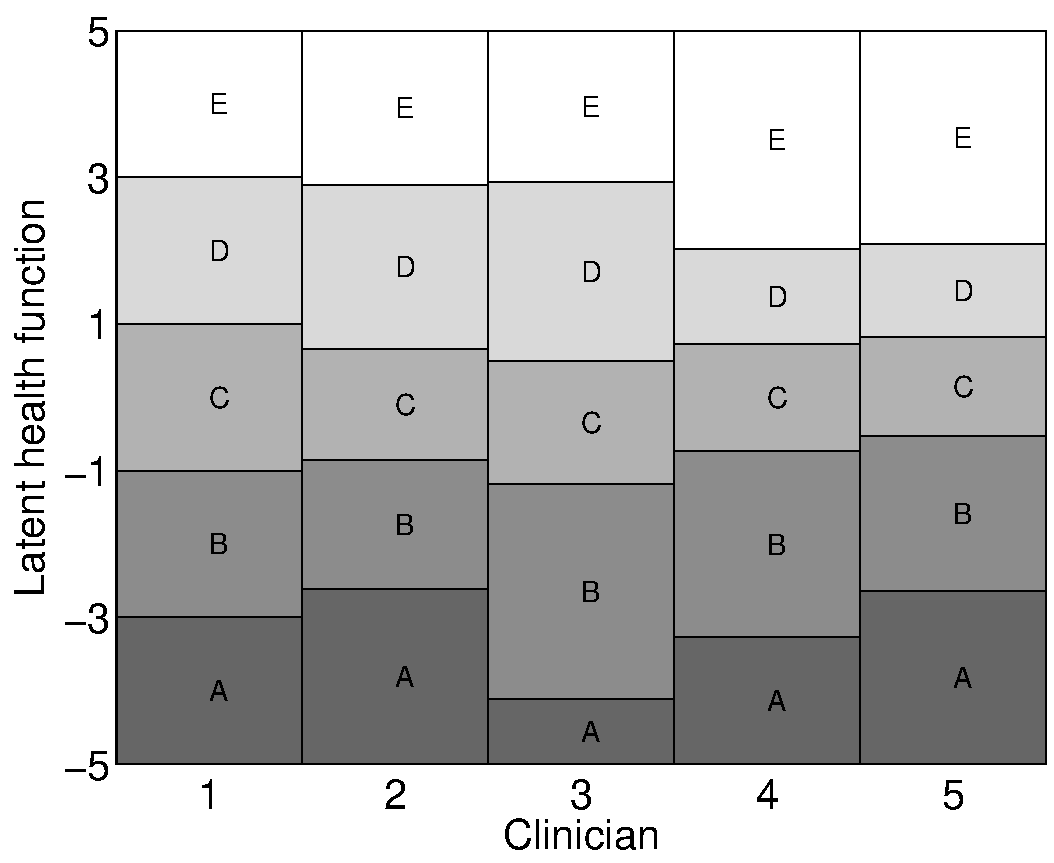
\includegraphics[width=0.45\linewidth]{end_thresh.pdf}}
		\centering\caption{\label{fig:clinicalcategories}Posterior mean cateogory boundaries.}
	\end{figure}
	\end{itemize}
\end{frame}

\begin{frame}
	\frametitle{Summary and Conclusions}
	\begin{itemize}
		\item Model allows us to:
		\begin{itemize}
			\item learn something about \emph{how} clinicians disagree and how they rate.
			\item assess the effectiveness of the INSIGHT procedure.
		\end{itemize}
		\item<2-> GP prior:
		\begin{itemize}
			\item Flexible
			\item Required no parametric assumptions about health function
			\item Hyper-parameter ($\gamma$) was inferred in the model (could be patient-specific)
		\end{itemize}
		\item<3-> Auxiliary Variable Trick:
		\begin{itemize}
			\item Not restricted to a standard Gaussian centered on the GP variable.
			\item Incorporated offset and precision without causing additional inference challenges.
		\end{itemize}
	\end{itemize}
\end{frame}

\mode<all>
% Dirichlet Processes
\lecture{Dirichlet Process Priors for Mixture Models}{Dirichlet}


\begin{frame}
	\frametitle{Mixture Models}
	\begin{itemize}
		\item A common strategy when faced with complex multi-modal data is to fit a \emph{mixture model}.
		\item In general:
		\[
			p(\bx) = \sum_{k=1}^K P(k)p(\bx|k)
		\]
		\item Where each component $p(\bx|k)$ is some simple density, e.g. Gaussian
		\item Within this model, we must know $K$ \emph{a-priori}
		\item Can do inference with Expectation-Maximisation, Variational Bayes, Gibbs Sampling, etc
		\item Generative process for $N$ data points:
		\begin{itemize}
			\item For each datapoint, $n$:
			\begin{itemize}
				\item Sample a component ($k$) according to $P(k)$.
				\item Sample $\bx_n\sim p(\bx_n|k)$
			\end{itemize}
		\end{itemize}
	\end{itemize}
\end{frame}

\begin{frame}
	\frametitle{Gibbs sampling for mixture models}
	\begin{itemize}
		\item Assume that the $k$th mixture component has parameters $\theta_k$.
		\item Define binary variables $z_{nk}$ where $z_{nk}=1$ if $n$th object is \emph{in} $k$th component and zero otherwise.
		\item Define $\pi_k = P(k)$.
		\item Define prior density on $\theta_k$: $p(\theta_k)$.
		\item For each iteration:
		\begin{itemize}
			\item Sample each $\theta_k$ from $p(\theta_k|\ldots) \propto p(\theta_k)\prod_n p(\bx_n|\theta_k)^{z_{nk}}$\\
			\item For each object $n$:
			\begin{itemize}
				\item Remove from its current component.
				\item Sample a new component: $P(z_{nk}=1|\ldots)\propto \pi_k p(\bx_n|\theta_k)$
			\end{itemize}
		\end{itemize}
	\end{itemize}
\end{frame}

\begin{frame}
	\frametitle{Being Bayesian}
	\begin{itemize}
		\item We should treat $\boldsymbol\pi = [\pi_1,\ldots,\pi_K]^T$ as a random variable.
		\item A suitable prior density is the Dirichlet:
		\[
			p(\boldsymbol\pi_k)  = \frac{\Gamma(\sum_k \beta)}{\prod_k \Gamma(\beta)}\prod_k \pi_k^{\beta_k-1}
		\]
		\item (from now on, we'll assume $\beta_k = \alpha/K~~\forall k$)
		\item<2->We will also assume that (\emph{a-priori}) the number of objects in each cluster ($c_k = \sum_n z_{nk}$) is multinomial with parameter $\bpi$:
		\[
			p(\mathbf{c}|\bpi) \propto \prod_k \pi_k^{c_k}
		\]
	\end{itemize}
\end{frame}

\begin{frame}
	\frametitle{Being Bayesian}
	\begin{itemize}
		\item We can now compute the posterior density for $\bpi$. It's another Dirichlet:
		\[
			p(\bpi|\mathbf{c},\alpha) =  \frac{\Gamma(\sum_k \alpha/K+c_k)}{\prod_k \Gamma(\alpha/K+c_k)}\prod_k \pi_k^{\alpha/K+c_k-1}
		\]
		\item<2->We can now also compute the probablity that some new observation would be placed in class $j$:
		\begin{eqnarray}
			\nonumber P(z_{*j} &=& 1|\mathbf{c},\alpha) = \int p(z_{*j}=1|\bpi)p(\bpi|\mathbf{c},\alpha)~d\bpi\\
			\nonumber &=& \int \pi_j p(\bpi|\mathbf{c},\alpha)\\
			\nonumber &=& \frac{c_j + \alpha/K}{\alpha + \sum_k c_k}
		\end{eqnarray}
		\item<2-> (Need to know that $\Gamma(z+1) = z\Gamma(z)$)
	\end{itemize}
\end{frame}

\begin{frame}
	\frametitle{Gibbs sampling again}
	\begin{itemize}
		\item Going back to our Gibbs sampling, we can replace $\pi_k$ with this expression:
		\[
			P(z_{nk}=1|\ldots)\propto \frac{c_k + \alpha/K}{\alpha + \sum_j c_j} p(\bx_n|\theta_k)
		\]
		\item Where the point being sampled shouldn't appear in any $c_j$ (i.e. $\sum_j c_j = N-1$)
	\end{itemize}
\end{frame}

\begin{frame}
	\frametitle{Sampling from the prior}
	\begin{itemize}
		\item We can ignore the data $\bx_n$ for a while and just sample partitions from this prior:
		\item Start with N objects, all in one cluster.
		\item For each iteration:
		\begin{itemize}
			\item For each object $n$:
			\begin{itemize}
				\item Remove from component it is in and re-assign with probability:
				\[
					P(z_{nk} = 1|\ldots) = \frac{c_k + \alpha/K}{\alpha + \sum_j c_k}
				\]
			\end{itemize}
		\end{itemize}
	\end{itemize}
\end{frame}

\begin{frame}
	\frametitle{Sampling from the prior}
	\begin{figure}[tbh]
		\centering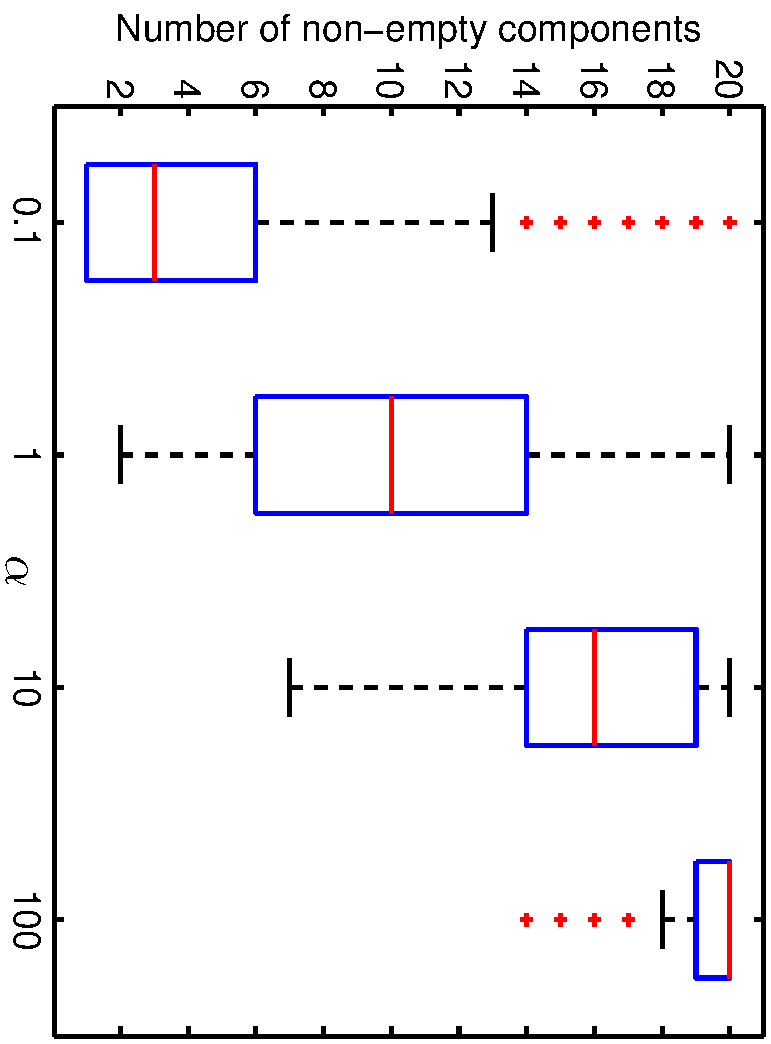
\includegraphics[height=0.8\linewidth,angle=90]{DPfixed.pdf}
		\centering\caption{\label{fig:dpfixed}Number of non-empty components as $\alpha$ is increased. $N=100$ and $K=20$. $\alpha$ controls how clustered the data are. Low $\alpha$ gives few populated clusters. Note: could have done this by sampling $\bpi$ and then sampling from $\bpi$)}
	\end{figure}
\end{frame}

\begin{frame}
	\frametitle{$K\rightarrow \infty$}
	\begin{itemize}
		\item What if we don't want to fix $K$?
		\item i.e. set $K=\infty$.
		\[
		P(Z_{nk}=1|\ldots) = \frac{c_k + \alpha/K}{\alpha + \sum_j c_j} = \frac{c_k}{\alpha + \sum_j c_j}
		\]
		\item This is the probability for one of the \emph{finite} number of clusters that are currently occupied.
		\item<2-> The probability of assigning to one of the \emph{infinite} number of unoccupied clusters must be:
		\[
		P(Z_{nk*}=1|\ldots) = 1 - \sum_k \frac{c_k}{\alpha + \sum_j c_j} = \frac{\alpha}{\alpha + \sum_j c_j}
		\]
		\item<3->A nice paper describing this: \href{http://www.gatsby.ucl.ac.uk/~edward/pub/inf.mix.nips.99.pdf}{Rasmussen 2000}
	\end{itemize}
\end{frame}

\begin{frame}
	\frametitle{Sampling from the $K=\infty$ prior}
	\begin{itemize}
		\item Start with $N$ objects all in one cluster
		\item For each iteration:
		\begin{itemize}
			\item For each object $n$:
			\begin{itemize}
				\item Remove from current component (if it leaves an empty component, delete it)
				\item Re-assign according to:
				\[
					P(z_{nk}=1|\ldots) = \left\{ \begin{array}{ll}
						\frac{c_k}{\alpha + \sum_j c_j} & \mbox{$k$ currently occupied}\\
						\frac{\alpha}{\alpha + \sum_j c_j} & \mbox{new $k$}
					\end{array}\right.
				\]
				\item if object in a new component, create one.
			\end{itemize}
		\end{itemize}
		\item<2->The prior we are sampling from is a \emph{Dirichlet Process}
	\end{itemize}
\end{frame}

\begin{frame}
	\frametitle{Sampling from the $K=\infty$ prior}
	\begin{figure}[tbh]
		\centering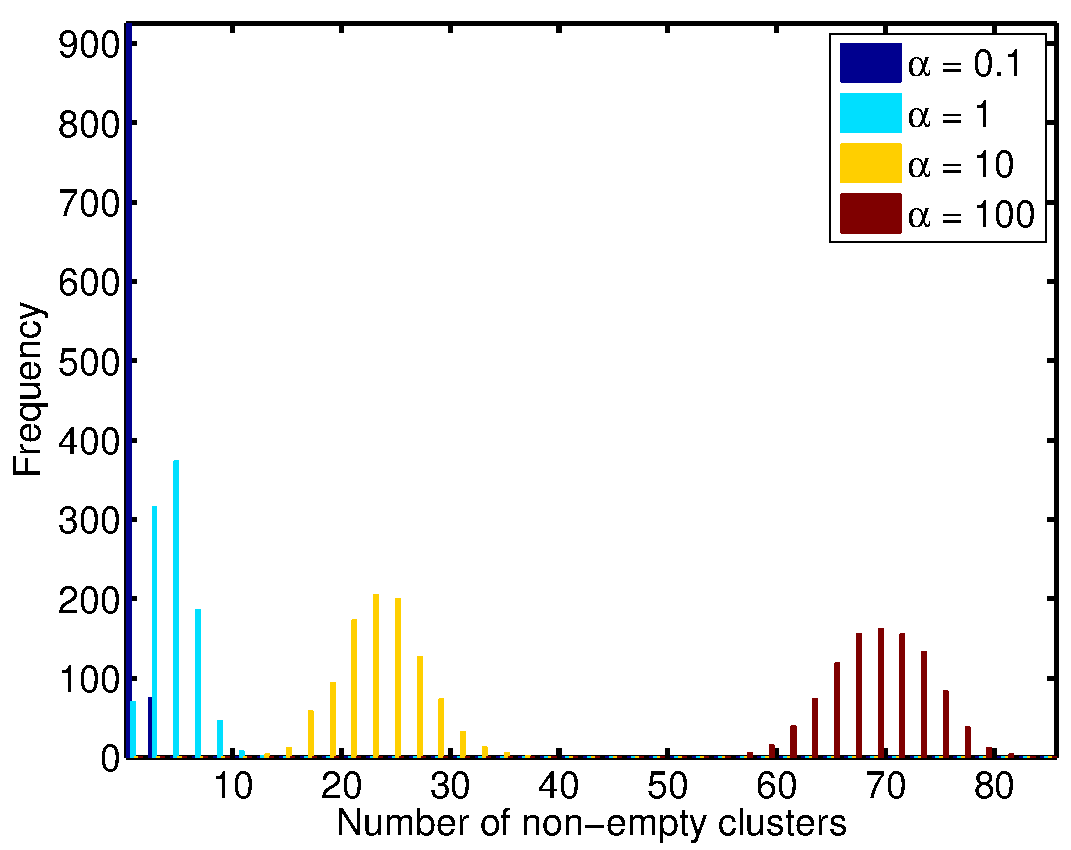
\includegraphics[width=0.8\linewidth]{DPbars.pdf}
		\centering\caption{\label{fig:DPbars}Number of non empty clusters as $\alpha$ is varied. $1000$ samples for $N=100$ objects.}
	\end{figure}
\end{frame}

\begin{frame}
	\frametitle{Including data}
	\begin{itemize}
		\item In general, we want to fit the model to objects $\bx_n$.
		\item Assume each component has parameters $\theta_k$.
		\item Assume a likelihood $p(\bx_n|\theta_k)$ and a prior $p(\theta_k)$
		\item<2->Gibbs sampling:
		\begin{itemize}
			\item Given a current clustering $\bZ$ and parameters $\theta_1,\ldots,\theta_k$
			\item For each object $\bx_n$ in each iteration:
			\begin{itemize}
				\item Remove $\bx_n$ from the model (might require deleting a component).
				\item Re-assign with probabilities:
				\[
					P(z_{nk}=1|\bx_n,\ldots)\propto \left\{\begin{array}{ll}
						c_k p(\bx_n|\theta_k) & \mbox{$k$ currently occupied}\\
						\alpha \int p(\bx_n|\theta)p(\theta)~d\theta & \mbox{new $k$}
					\end{array}\right.
				\]
				\item Sample $\theta_k$ for each component:
				\[
				p(\theta_k|\ldots)\propto p(\theta_k)\prod_n p(\bx_n|\theta_k)^{z_{nk}}
				\]
			\end{itemize}
		\end{itemize}
		\item<3->If everything conjugate, can integrate $\theta_k$ out completely (better convergence).
	\end{itemize}
\end{frame}
\begin{frame}
	\frametitle{\ac{CRP}}
	\begin{itemize}
		\item A popular way of thinking about DPs is via the `Chinese Restaurant Process'
		\item Prior:
		\begin{itemize}
			\item $N$ people enter a Chinese Restaurant with infinite tables.
			\item The first person sits at the first table.
			\item The $n$th person sits at an occupied table with probability proportional to the number of people already at the table, or a new table with probability proportional to $\alpha$.
		\end{itemize}
		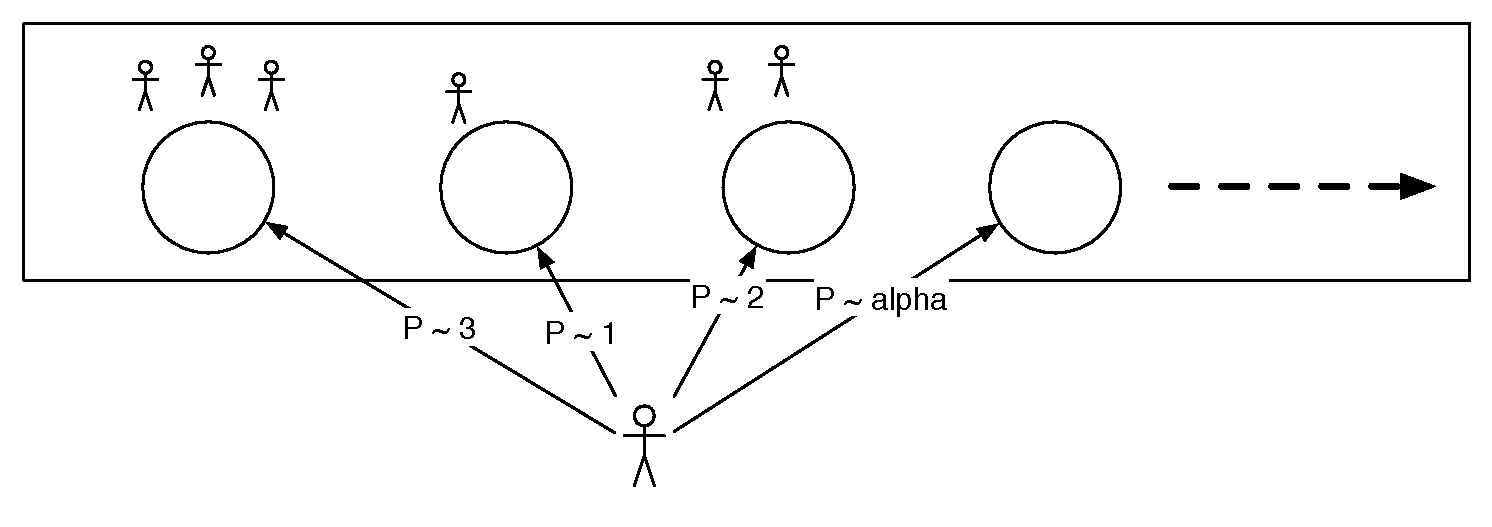
\includegraphics[width=\linewidth]{CRP.pdf}		
	\end{itemize}
\end{frame}

\begin{frame}
	\frametitle{\ac{CRP}}
	\begin{itemize}
		\item With data:
		\begin{itemize}
			\item Each table has one dish. Table choice also depends on dish preference.
			\item Table dishes updated according to preference of people at table (here the analogy starts(!) to get a bit tenuous)
		\end{itemize}
		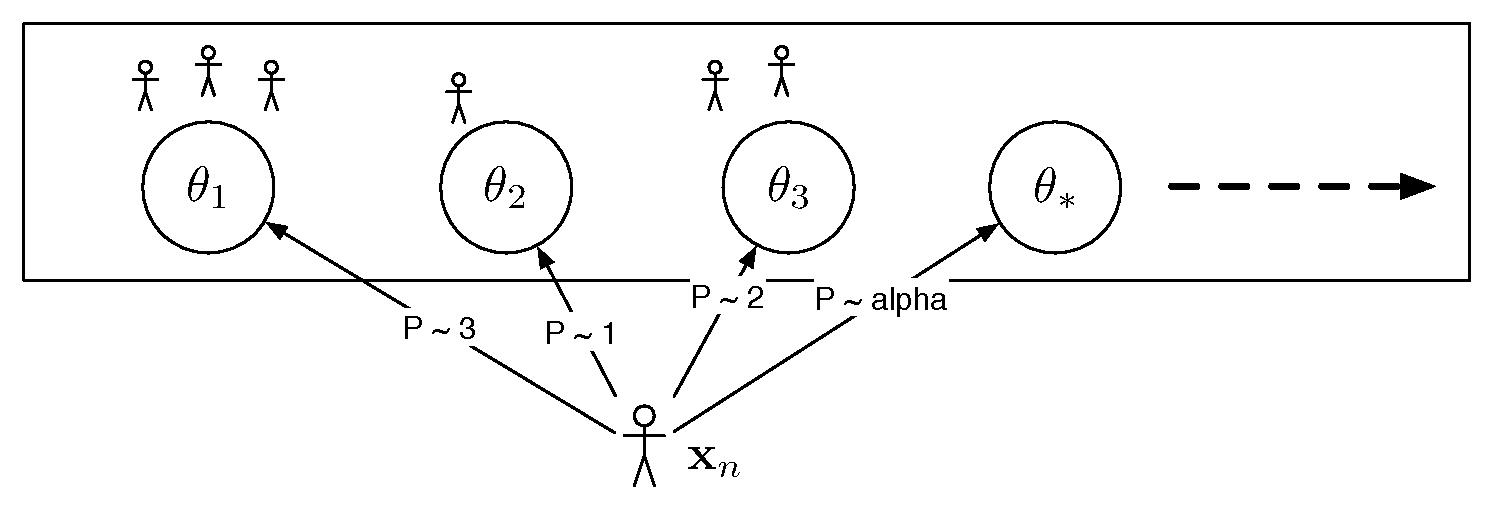
\includegraphics[width=\linewidth]{CRP2.pdf}
	\end{itemize}
\end{frame}

\begin{frame}
	\frametitle{Example}
	\begin{figure}[tbh]
		\centering\includegraphics<1>[width=0.8\linewidth]{CRP_data.pdf}
		\centering\includegraphics<2>[width=0.8\linewidth]{CRP_sim.pdf}
		\centering\includegraphics<3>[width=0.8\linewidth]{CRP_K.pdf}
		\centering\caption{\label{fig:CRP_example}Example output from CRP with Gibbs sampling. The data has three clusters. Visualising the $\theta_k$ is impossible, but we can look at the probablility that two objects are in the same cluster, and the number of clusters.}
	\end{figure}
\end{frame}

\mode<all>
% Metabolomics

\lecture{A mixture model for metabolite peak identification}{Metabolomics}

\begin{frame}
	\frametitle{Metabolomics}
	\begin{itemize}
		\item Metabolome: the set of small molecule metabolites found within an organism.
		\begin{itemize}
			\item Hormones, sugars, etc 
		\end{itemize}
		\item Gives a reliable picture of the phenotype (\href{http://www.nature.com/ng/journal/v41/n2/abs/ng.308.html}{Fu et al 2009})
		\item But metabolites are hard to measure.
		\item Dominant paradigm is \ac{LC} \ac{MS}
	\end{itemize}
\end{frame}

\begin{frame}
	\frametitle{\ac{LS}/\ac{MS}}
	
\end{frame}

\mode<all>
% hdp
\lecture{The Hierarchical Dirichlet Process}{hdp}

\begin{frame}
	\frametitle{The Hierarchical DP}
	\begin{itemize}
		\item Imagine we have $>1$ related dataset to cluster, generated by the same process
		\item Fitting separate mixtures to each results in a loss of information
		\item The \ac{HDP} allows them to be analysed together with shared parameters
		\begin{itemize}
			\item e.g. datasets clustered individually but cluster parameters (e.g. means) can be \emph{shared}
			\item Analogy: The Chinese Restaurant Franchise
			\item Described in \href{http://www.cs.berkeley.edu/~jordan/papers/hdp.pdf}{Teh et.~al}
		\end{itemize}
	\end{itemize}
\end{frame}

\begin{frame}
	\frametitle{The Chinese Restaurant Franchise}
	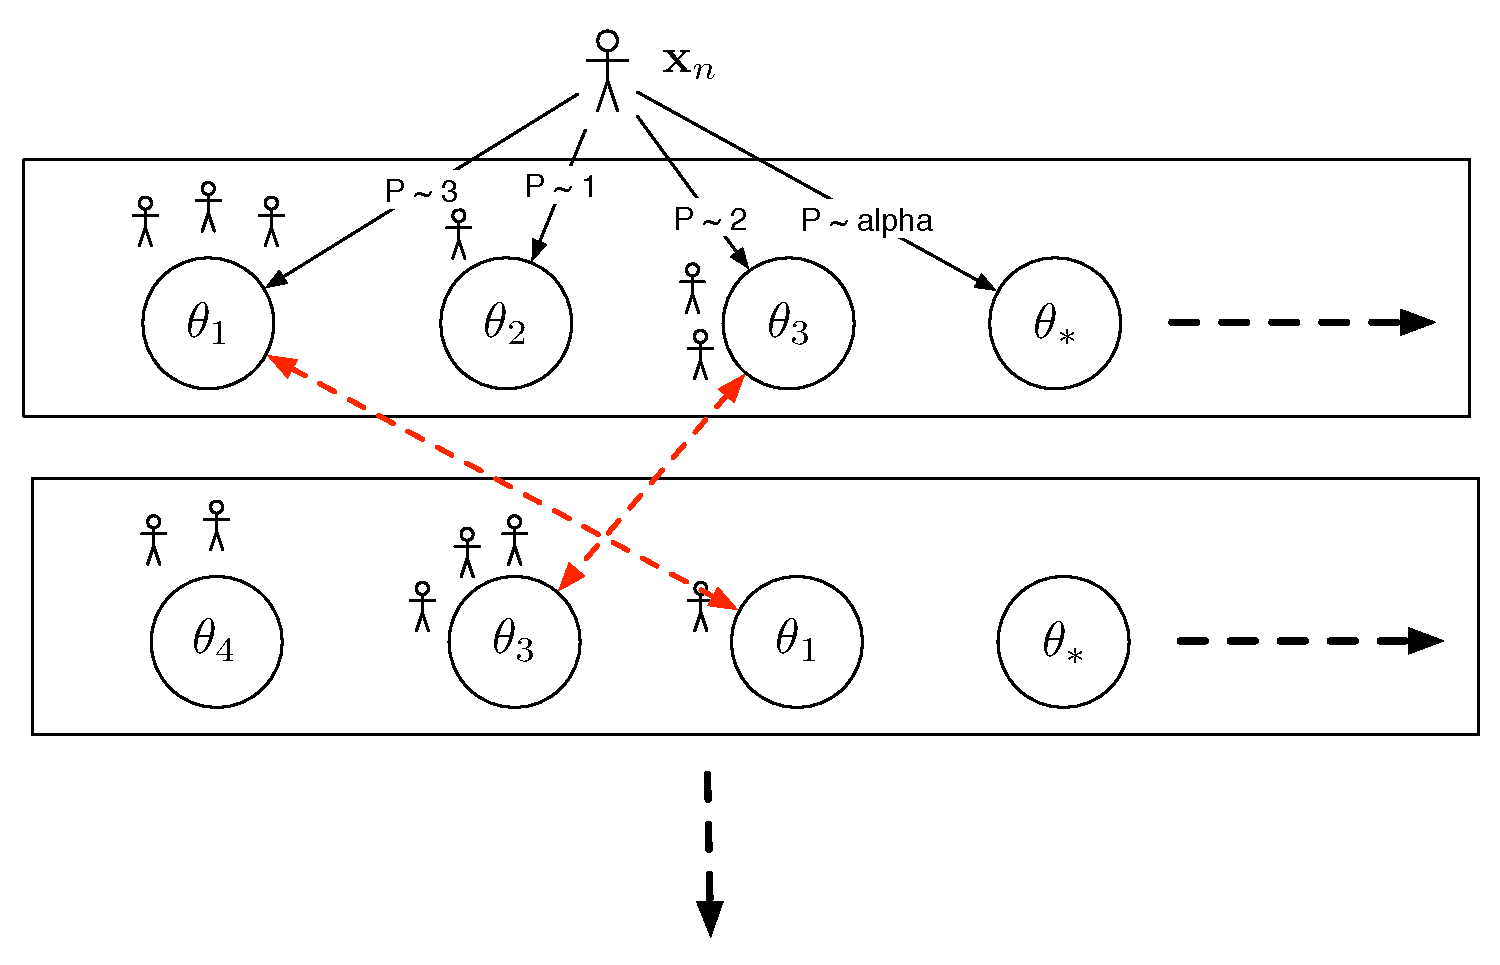
\includegraphics[width=\linewidth]{CRPfranchise}
\end{frame}

\begin{frame}
	\frametitle{The Chinese Restaurant Franchise}
	\begin{itemize}
		\item Gibbs sampling is very similar to the single restaurant case
		\item Each object is re-assigned to a table with probabilities ($i$ indexes datasets):
		\[
			P(z_{ink} = 1|\ldots)\propto \left\{
			\begin{array}{cc}
				n_{ik}p(\bx_{in}|\theta_k) & \mbox{for current table}\\
				\alpha p(\bx_{in}) & \mbox{for new $k$}
			\end{array}
			\right.			
		\]
		\item $p(\bx_{in})$ is computed by marginalising all possible values for the parameters at the new tables.
		\begin{itemize}
			\item These include values used for current tables (with prior proportional to the number of tables they're used at) and a completely new value (with prior proportional to, say, $\gamma$).
			\item i.e. There are \ac{DP}s for assignment of objects to tables and assignment tables to parameters.
		\end{itemize}
	\end{itemize}
\end{frame}

\begin{frame}
	\frametitle{Data sampled from a \ac{HDP}}
	\begin{multicols}{2}
		\centering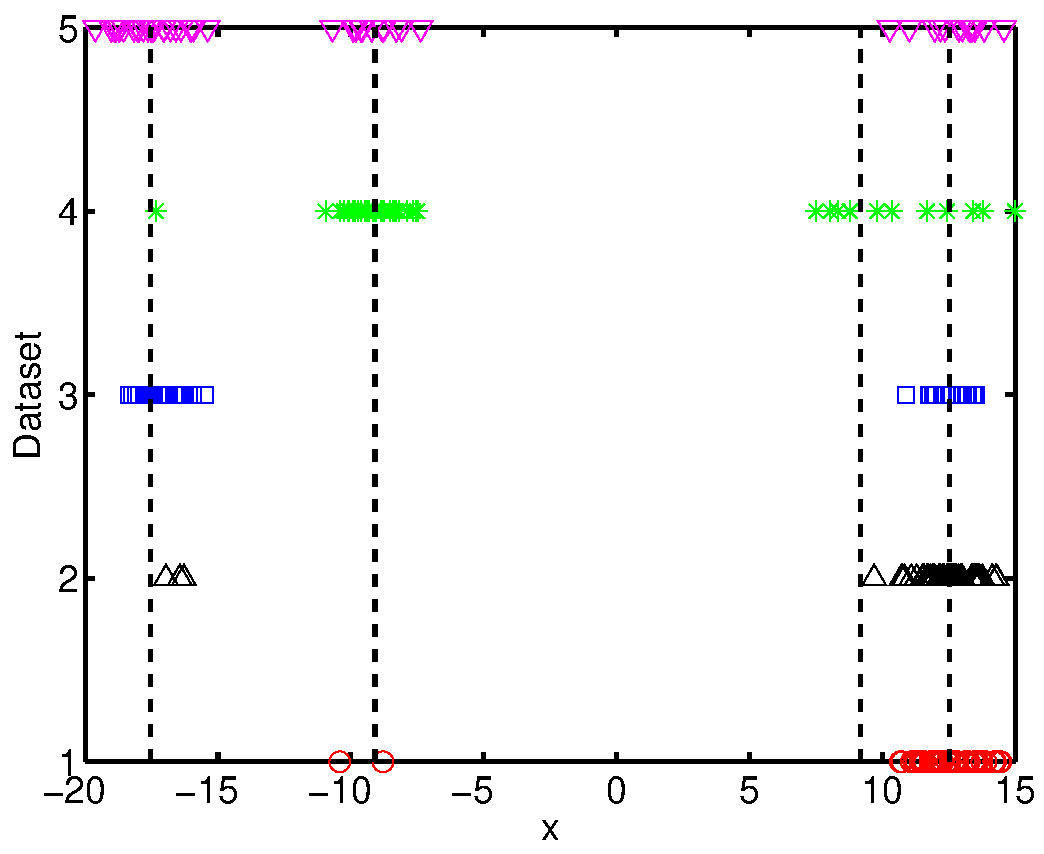
\includegraphics[width=\linewidth]{hdp_data}
		\newpage
		\begin{itemize}
			\item 5 datasets
			\item 4 top level components (dashed line)
			\item Each data has data from a subset of components
		\end{itemize}
	\end{multicols}
\end{frame}

\begin{frame}
	\frametitle{\ac{HDP} inference example}
	\begin{multicols}{2}
	\begin{itemize}
		\item 300 posterior samples.
		\item Does pretty good job.
		\item At last sample, posterior means over top-level components were: 12.5215, -17.0304, -9.0535, 8.7857, -17.5636, -16.12
		\item True: [12.5185,-9.0909,-17.5295,9.1839]
	\end{itemize}
	\newpage
	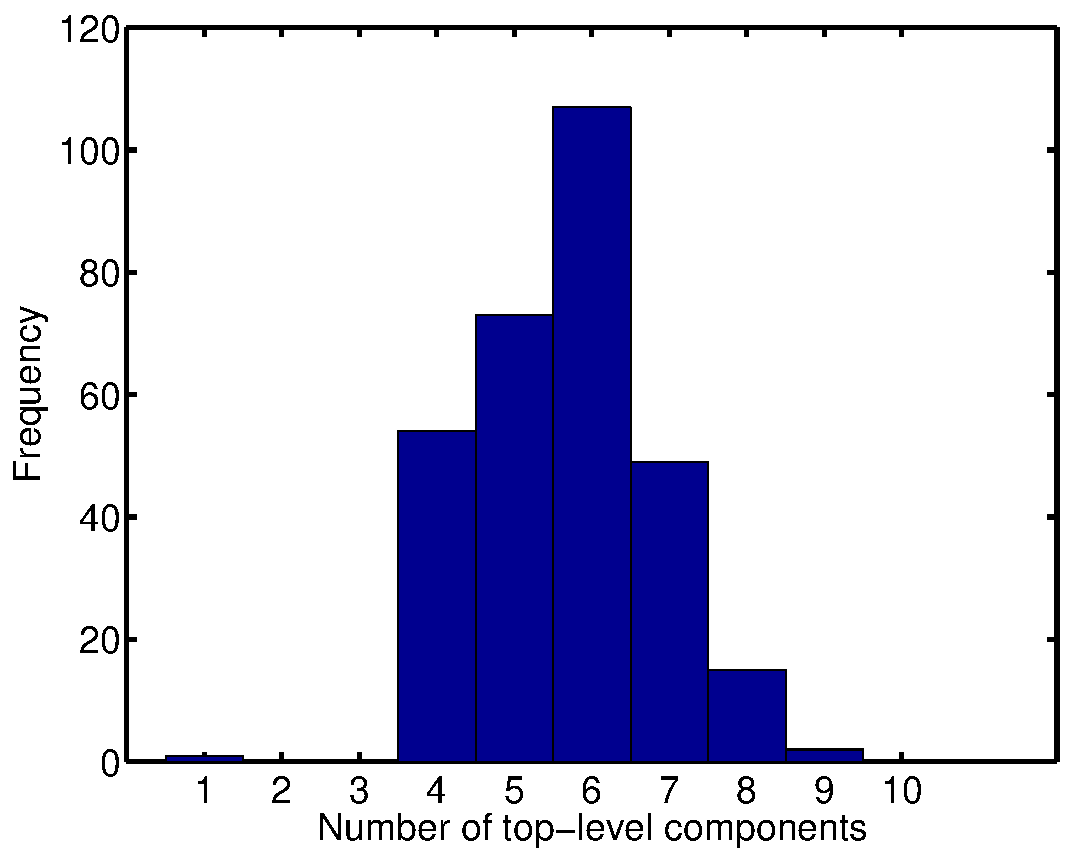
\includegraphics[width=\linewidth]{hdp_inference}		
	\end{multicols}
	\begin{itemize}
		\item Note that mixing would be improved by also re-sampling assignment of clusters to top components.
	\end{itemize}
\end{frame}

\end{document}